\documentclass[8pt]{article}
\title {Quantifying the uncertainty around the spreading of COVID-19 in
Italy and Germany}

\usepackage{graphicx}
\usepackage{verbatim}
\usepackage{amsthm}
\usepackage{amssymb}
\usepackage{amsmath}
\newtheorem{deff}{Definition}
\usepackage{graphicx}
\usepackage{subcaption}
\usepackage[font=small,labelfont=bf]{caption}


\newcommand{\norm}[1]{\left\lVert#1\right\rVert}
%\newtheorem{theorem}{Proposition}
\newtheorem{definition}{Definition}
\newtheorem{Proposition}{Proposition}

\begin{document}
\maketitle
\section{Introduction}
When modeling the Coronavirus evolution, one aims at
finding the function $X(t)$ describing some data running in time,
like the number of infected or deceased people, to make then
future predictions.
One needs to assume the belonging of $X$ to some family of functions
described by $n$ real parameters to estimate through 
the observation of empirical measurements.
By collecting them into a vector $P \in \mathbb{R}^n$, 
we stress the dependence by writing $X(t) = X^P(t)$ when needed.


Instead of looking for precise value of $P$, we adopt a probabilistic
viewpoint when we embrace an \emph{uncertainty} around it, quantified
by using Bayesian techniques. Then, by choosing the parameters corresponding
to the "worst" and the "best" scenario, we draw curves in time, delimiting the
area in which we expect the future data to oscillate.


Dealing with the model's choice for $X$, 
we recall that many epidemiological models are given by autonomous ODEs. 
This is for instance the case of
SIS and their related, as well as of general logistic maps.
After pointing out a connection between these two common classes,
we explain in detail our choice in favor to the latter.


When moving on concrete simulations for Germany and Italy,
we clearly point out all the taken assumptions and
remark the importance of the right choice for a dataset,
the influence of lockdown effects on that,
and how the ODE semigroup property might be helpful in that regard.


\section {The use of logistic models}
\subsection {Introduction}
One of the simplest idea for epidemiological modeling is to divide the
number of total existing people $N$, 
into two classes $S(t)$ and $I(t)$, such that
their sum $S + I = N$ is constant over time. People switch dynamically from
the set $S$ of \emph{susceptible}, to $I$ of \emph{infected}, and
conversely. Observe how in this model there are no fatal cases,
but this does not represent a problem since we take it just as a
starting point.
This simple scheme is known under the name of SIS and
governed by a system of two ODEs:

\begin{equation}
\begin{cases}
	S'(t) = - \beta S(t) I(t) + \alpha I(t) \\
	I'(t) = - \alpha I(t) + \beta S(t) I(t) \\
\end{cases}
\end{equation}


A complete explanation about the interpretation and the ideas beyond can be
found in REF, but for us it now important to remark how $\beta$ and $\alpha$
have specific interpretations. Beta is connected to how many 
people randomly meet per unit of time,
while $\frac{1}{\alpha}$ is the mean time required to heal. 


Since the sum $S + I = N$ is constant over time, a substitution
into the ODE leads to the simple logistic equation governing the number of
actively infected:

\begin{equation}
	I' (t) = r I(t) \left (1 - \frac{1}{K} \right)
\end{equation}
where $r = \beta N - \alpha$ and $k = N - \frac{\alpha}{\beta}$.


The equation above belongs to the family of logistic functions, maps
in principle not specifically connected to epidemiology. They are curves
obtained as solution of one dimensional
autonomous ODEs, with S-shaped trajectories starting with an exponential
growth, gradually stopped, until reaching an horizontal constant phase.


We chosen them as a prototype model for our simulations,
justified by the intuition that if the simplest compartmental
epidemiology model (SIS) is equivalent to the simplest logistic map,
then by choosing more general logistic functions we might implicitly
work with more realistic epidemiological models.
Furthermore, we do not model the number of actively infected,
but rather the amount of total infected and number of deaths.
We ignore further theoretical analysis for this decision,
we kept the choice encouraged by nice concrete results.

\subsection {The generalized logistic map: Richard's ODE}
The most general logistic map (still expressed by an ODE,
 we'll see later the reason beyond this requirement)
is given by the Richard's equation.
It's the following ordinary differential equation governed by
three real positive parameters, 
$P = \{ q, Q, \nu \}$, so $n = 3$. We need to fix an initial condition $X_0$
(not considered as parameter since directly observed from data),
and write the model as $X(t) = X^P(t) = X^P_{X_0}(t)$
when we want to stress this dependence.
The Richard's law satisfy the equation:

\begin{equation}
	X'(t) = q X(t) 
	\left ( 1 - \left( \frac{X(t)}{Q} \right)^{\nu}\right )
\end{equation}
with closed form solution:
\begin{equation}
	X(t) = \frac{Q} { (1 + A \exp[-q \nu t])^{\frac{1}{\nu}}}
\end{equation}

Here $A$ is just an abbreviation  for
$A = -1 + \left ( \frac{Q} { X_0} \right )^{\nu}$.
The parameter $\nu$ is related to the symmetry of the curve,
while $q$ represents the initial exponential growth then stopped
in time. Intuitively we think of it to be related to the
average amount of people's social contacts, as in the simpler logistic case
connected to the SIS model.


By taking the limit $\lim_{t \to \infty} X(t) = Q$, 
we understand $Q$ to represent the asymptotic maximal value.


Setting $\nu = 1$ gives the basic logistic map, described
in the next section, while taking the limit $\nu \mapsto 0$ 
under appropriate gives the Gompertz law, explained later.



\subsection {The simple logistic map}
In the simple logistic map the model $X^P(t)$ depends on two real positive
parameters, $P = \{ q, Q \}$, so that $n = 2$,
and is the solution of the 1-dimensional ODE:
\begin{equation}
	X'(t)  = q X(t) \left ( 1 - \frac{X(t)}{Q} \right )
\end{equation}
with closed-form formula:
\begin{equation}
X(t) = \frac{X_0 \exp[q t]}
	{1-\frac{X_0}{Q} (1-\exp[q t)])}
\end{equation}


Where again $X_0$ is the starting ODE condition at time $0$.
Of course, we have $\lim_{t \to \infty} X(t) = Q$,
and since this simple logistic map is equivalent to the simplest SIS
model (as explained before), the parameter $q$ can be actually
rigorously related to the average number of daily people's social interaction.


\subsection{The Gompertz law}
The Gompertz law is governed by two real positive parameters,
$q$ and $Q$, therefore we write again $P = \{q, Q\}$ and $n = 2$.
Once the starting condition $X_0$ at time zero
is specified, $X(t) = X^P(t) = X_{X_0}^P(t)$ is the solution to:

\begin{equation}
 X'(t) = q X(t) \log \left [\frac{Q} {X(t)} \right ]
\end{equation}
expressed by the closed-form formula:
\begin{equation}
X(t) = Q \exp	\left [
	\log \left [ \frac{X_0}{Q} \right ]
	\exp \left [ -q t \right ]
		\right ]
\end{equation} 


As seen for the previous cases, $Q$ corresponds to the limit
$\lim_{t \to \infty} X(t)$.


\section {The bayesian approach}
When using the models above in practice, we can only observe a
limited amount of points coming from the ODE trajectory, 
perturbed by a random noise.
Let's fix $T+1$ times $\{t_i\}_{i = 0,\dots, T}$.
\begin{definition}
	The \emph{observed vector} $\textbf{y} \in \mathbb{R}^{T+1}$
	is the random variable defined componentwise as:

\begin{equation}
	y_i(\omega) = X^P_{X_0} (t_i) + \eta_i(\omega)
\end{equation}
\end{definition}
We assume the error expression 
$\eta_i \sim \mathcal{N}(0, \sigma^2_i)$ with a time dependent variance.
Sometimes by an abuse of notation 
we use the symbol $\eta_i$ to indicate its density function too,
so writing $\eta_i(x)$ for $x \in \mathbb{R}$ refers to that.


Recall that the finally goal is to give an estimation
of the unknown values for $P \mathbb{R}^n$,
\emph{given} the observation $\textbf{y}$.
We choose a Bayesian approach to find a solution. Therefore, we need
to define a prior distribution for $P$, a likelihood function,
then we get the solution as the product of them.
In other words,
during the search for the true parameters, $P$ is seen as a random
variable $\Omega \to \mathbb{R}^n$ whose law, 
\emph{conditioned} on the observations,
is what we aim to understand.


As standard in the field, we start by assuming that
$\mathbb{P}[ P \in A] = \rho(A)$ is described by a specific 
density function $\rho$ called the prior distribution, 
representing our blind guess about $P$ \emph{independently} of the 
observations $\textbf{y}$.


If we aim at understanding 
$\mathbb{P}[P | \textbf{y}]$, then the classical Bayes's law allows to find
it in terms of an hypothetical law $\mathbb{P}[\textbf{y} | P]$: this
is where the notion of likelihood comes into play.


\begin{definition}
For every fixed choice of the parameters $P$, the likelihood functions
for the observation of $\textbf{y}$, given $P$, is defined to be:
	\begin{equation}
	\mathcal{L}(\textbf{y}|P) \doteq 
		\frac{(2 \pi)^{- \frac{T}{2}}}
		{\sigma_0\dots\sigma_{T}}
		\exp \left( -\frac{1}{2} 
		\sum_{i=0}^{T} 
		\frac{(y_i - X_{X_0}^P(t_i))^2}
		{\sigma_i^2}
		\right )
	\end{equation}
\end{definition}


By \emph{interpreting} the likelihood as an effective probability
conditioning, writing informally 
$\mathbb{P}[\textbf{y}|P] = \mathcal{L}(\textbf{y}|P)$,
its formula is then explained when looking at the noise
distribution $\eta(\textbf{y} - X^P)$.
By imitating the Bayes's rule:
\begin{equation}
\mathbb{P}[P | \textbf{y}] \propto
	\mathbb{P}[\textbf{y} | P] \mathbb{P}[P]
\end{equation}
the final result is defined as:

\begin{definition}
	The (Bayesian)
	answer to the problem "find the probability density of
	the parameters $P$ given the observations $\textbf{y}$"
	is given by the \emph{posterior}
	distribution on $\mathbb{R}^{n}$ defined by:
	\begin{equation}
		\mu(dx) \propto \mathcal{L}(\textbf{y} | x) \rho(dx)
	\end{equation}
\end{definition}


During every use of the Bayesian rule, we constantly omitted the denominator
term relying always on the mere proportionality "$\propto$". 
This because such a value is always the probability 
normalization constant,
a number that can be completely ignored in practice thanks to the use
of suitable numerical techniques.


In few words, this section should have transmitted the idea that
the problem 
"estimating the parameters $P$" 
has been converted into the problem 
"understanding the probability distribution $\mu$".



\begin{comment}
\section {The Bayesian approach}
\subsection {Inverse Bayesian problems}
As a general formulation, the inverse problem 
consists on having a known borelian \emph{observation operator}
$G: \mathbb{R}^n \to \mathbb{R}^m$, an \textbf{unknown} 
input $x \in \mathbb{R}^n$ to be found from
a known \emph{measurement} $y = G(x) + \eta$, where $\eta$ is a centered
gaussian random variable, called the noise, with some specified variance.
With an abuse of notation we use $\eta$ for its gaussian
density function, too, justifying the writing 
$\eta(u)$ for $u \in \mathbb{R}^m$.


In other words we are interested in performing an indirect estimation 
(the value $x$) from a noised direct measurement $y$
through the use of a model $G$.
A \emph{lot} of theoretical issues are here into play. To mention
few of them, the map $G$ might admit different preimages, none at all,
or the noise might send $y$ outside the range of $G$.
Some of these problems are circumvented by minimizing appropriate distances
$\norm{G(x) - y}$ instead, but they might be insufficient or too hard.
For instance, distance minimization is precisely the technique used
for the classic least square minimization.


In support on the described challenge,
switching to a probabilistic mindset can offer a precious support.
Observe the conditioned distribution induced from the noise:
\begin{equation}
	\mathbb{P} [ y | x] = \eta(y - G(x))
\end{equation}

The probability measure above is called the \emph{likelihood} and,
by construction, is simply a gaussian centered on the true
value of $x$.
When the variance is small, the probabilistic search for $x$ 
is a relatively easy process, being $x$ the unique solution
that maximizes the probability.
But when the noise is increased,
the bell enlarges making harder to distinguish the "true" $x$
from points in its neighborhoods, who share now very high
probability values.
Theoretically $x$ is still unique, but in practice the interval
of uncertainty is much larger.

In the bayesian approach we start from these remarks,
but we also suppose to have a belief about the true value of $x$,
by choosing a probability distribution $\rho$ on the domain
$\mathbb{R}^n$ called the
\emph{prior}.
Then we rely on the Bayes formula:

\begin{equation}
\mathbb{P}[x | y] = \frac{ \mathbb{P}[y | x] \mathbb{P}[x]} {\mathbb{P}[y]}
\end{equation}

to define the \emph{posterior} distribution, still on the domain
$\mathbb{R}^n$, as:
\begin{equation}
\mu (x) \doteq \mathbb{P}[x|y] = \frac{ \eta(y - G(x)) \rho(x)} {\mathbb{P}[y]}
\end{equation}


Since the point $y$ is fixed, the denominator is just the normalization
constant than we can ignore thanks to suitable numerical methods.


The measure $\mu$ is the mathematically
formalization of the idea: "the best that we can say (about $x$) starting
from a certain belief ($\rho$) and (noised) concrete observations ($y$)".


We define $\mu$ to be the solution of the inversion problem.
Its statistical properties will say a lot about the uncertainty around
the true input $x$. Under certain conditions (see REF), it can be shown that
the distribution $\mu$ converges to a Dirac's delta when the noise's variance
goes to zero, with such a delta centered on the same point resulting
from a (regularized) least square minimization. This is why we can interpret
the Bayesian approach as an \emph{extension} capable of managing the error's
influence more naturally. 


Finally, when using least squares to detect a
parameter on $\mathbb{R}^n$ in presence of noise, 
one generally obtain an interval on confidence/uncertainty on each coordinate. 
Conversely, the Bayesian algorithm offers directly a probability
distribution on the whole $\mathbb{R}^n$ that can be used to detect possible
correlations between the parameters uncertainty: for instance, in the later
numerical results concerning the Coronavirus modeling,
the posterior's distributions have usually a "banana shape": therefore
accepting some degree of uncertainty around a single coordinates 
will force the the uncertainty around the remaining.
\end{comment}


\subsection{The pCN Monte Carlo algorithm}
In the previous section we explained the Bayesian strategy to convert
the problem of parameter estimation to
the understating of the posterior probability measure $\mu$.
In principle it could be possible to detect various properties
by using analytical tools, but due to time constraints we rely on a simple
effective strategy: first produce a large amount of samples from $\mu$,
then analyze them statistically.


The chosen algorithm is the preconditioned Crank-Nicolson
Monte Carlo (pCN), in general particularly strong on high
dimensional spaces and capable of managing well discretizations
coming from infinite dimensional Gaussians.
Here we briefly revise and adapt it for our specific
and much simpler situation. The pCN algorithm \emph{requires}
the choice of a Gaussian prior distribution $\rho$.


Recall that $n$ is the carnality of $P$ (so, $2$ or $3$
according to the chosen model). For two points in $\mathbb{R}^n$,
define the choice probability:

\begin{equation}
	a(u, v) \doteq \min \{ 1, \frac{ \mathcal{L}(\textbf{y} | u )}
				{\mathcal{L}(\textbf{y} | v)} \}
\end{equation}
and set the \emph{exploratory} parameter $0 < \beta_{pcn} < 1$ 
(see step 3).


To produce a \textbf{single sample} from $\mu$, construct a chain 
$\{ x_i \} _{i \in \mathbb{N} }$ as follows:

\begin{enumerate}
	\item set $x_0 \in \mathbb{R}^n$ arbitrarily. Then, for each
		$k > 0$:
	\item sample a point $R$ from the gaussian prior distribution $\rho$;

	\item  propose a candidate as 
		$
		\hat{x}_{k} = \sqrt{(1 - \beta^2)} x_{k-1}
			+ \beta R
		$;
	\item	accept it (i.e. set $x_{k} = \hat{x}_{k}$)
		with probability $a(x_{k-1}, \hat{x}_k)$;
	\item (accepted or not) repeat from 2;
\end{enumerate}
We define $N_{pcn}$ the integer at which we always stop the chain,
producing therefore a single approximated posterior's sample.
Of course repeating the algorithm allows to collect 
a large amount of sample (define this number as $S_{pcn}$),
and we remark how every instance is
independent and therefore suitable to parallelization
(the user must be warned about the use of a proper seed).

\begin{comment}
\subsection{The k-means algorithm}
TO REWRITE
Once we have a large set of samples from the posterior distribution
(usually more that $5000$ points each of dimension $n$, where 
$x \in \mathbb{R}^n$, i.e. $n$ is the number of parameters to estimate),
we want to actually understand how to use this information.
Therefore we need a strategy to reduce the dimension.
We borrow a simple but strong technique
from the Machine Learning community, called the \emph{k-means} algorithm.


In few words given a cloud of points in $\mathbb{R}^n$, the k-means allows
to divide it in a selected number of \emph{clusters}, call it $k$,
each represented
by a \emph{centroid}. You can think on this algorithm as a multidimensional
way of performing an histogram. Therefore, as for the latter case,
there is no fixed-universal rule for the right amount of centroids.
More regular distributions are likely to be represented well with a few
numbers of them, and for our application we found $k = 5$ to be a fair choice. 
It means than for each observation (dataset) we will have $k$ 
predictions for the same model, each with an associated probability rate.
We underline how this uncertainty comes from the fact of considering
the noise as an intrinsic element of the problem itself.
\end{comment}

\begin{comment}
\subsection {Using Bayesian Inversion as interpolator}
It is now time to connect together the bayesian theory explained above
with our equations for the spreading of the Coronavirus.

Let's consider a model $X_{X_0}^P(t)$ belonging to a class
described in the first section. 
Recall, this is the trajectory of a 
logistic-like ODE (basic, Richard or Gompertz)
starting with initial condition $X_0$ at time $0$ and depending on
appropriate parameters $P \in \mathbb{R}^n$ ($n = 2, 2, 3$ respectively).


Let's fix a time horizon $T$ and consider
the points $X_{X_0}^P(t)$, for days $t \in \{0, 1, \dots, T\}$.
Note that, by construction, they are  
the number of infected in these $T+1$ days according to the model.


Since we are interested in deducing $P$ 
from the empirical noised observation of the values above,
we are come back to the bayesian inversion context by defining:
$G : \mathbb{R}^n \to \mathbb{R}^{T+1}$, in the section above,
as the map
$P \mapsto \{X_0, X_{X_0}^P(1), \dots, X_{X_0}^P (T)\}$.


\begin{comment}
\section{Criteria for a reliable prediction}
Let's suppose to have a model given by an autonomous
ODE, a dataset with days and values,
and the problem of estimating the ODE parameters $P$ from them.
We use a technique to interpolate (like the Bayesian one
explained before), we obtain results (like the posterior
probability measure), and the implicit question is:
how should these results be read?
Are there some criteria to ensure more reliability?
In this section we point out general remarks, and for each of them
we show their effect on the posterior's distribution behavior.
This is an essential prerequisite to ensure the correct
interpretation of true numerical results, showed in the next final section.
\end{comment}

\begin{comment}
For sure a requirement is to produce a "small enough" interpolation error.
A second step might be to split the dataset into two parts, using part
of it to train the model (i.e. estimate $P$),
and the remaining to compare with the just obtained prediction,
(the common \emph{cross-validation}). 
We propose a further requirement
merely depending on the fact of working with simple autonomous ODE,
by considering the semigroup property of its associated
flow.
\end{comment}

\begin{comment}
\subsection{Interpolation error}
We start with the easiest notion, for the sake of fixing some notation.

\begin{definition}
	A \emph{dataset} $\mathcal{D}_{k, T}$ from day $k$ to day $T$
	is a collection of $T - k + 1$ couples,
	$\mathcal{D}_{k, T} = \{(n, V_n)\}_{k \leq n \leq T}$.
\end{definition}


We think of it always as "day, value at that day".
In particular, it can correspond to a discrete ODE trajectory:
\begin{definition}
	A dataset $\mathcal{D}_{k,T}^P$ is said to \textbf{fulfill}
	an ODE, $X^P(t)$, for some fixed set of parameters $P$,
	if when $V_k$ is chosen as starting condition
	for $X^P$ at time zero, we have:
\begin{equation}
	V_{k + i} = X_{V_k}^P(i) \quad \forall 1 \leq i \leq T
\end{equation}
	in such a case we write $V_k = V_k^P$ to point out the dependency.
\end{definition}


Note that modeling a dataset with $X^P$ is precisely the same as
understanding if there exists a $P$, such that 
$\mathcal{D} = \mathcal{D}^P$. It justifies the notion of interpolation
error.
\begin{definition}
	Let $\mathcal{D}^P_{k, T}$ be a dataset fulfilling an $X^P(t)$.
	Let $\mathcal{D}_{k, T}$ be an empirical collection of data.
	The (relative percentage) interpolation error between
	the two is defined as:
	\begin{equation}
		\norm{\mathcal{D}^P_{k,T} - \mathcal{D}_{k,T}}_{err} 
		\doteq 100 \frac
		{\sum_{n=k}^{T} |V^P_n - V_n|^2}
		{\sum_{n=k}^{T} |V^P_n|^2}
	\end{equation}
\end{definition}

Therefore is clear that 
if $\mathcal{D} = \mathcal{D}^P$ for some parameter $P$, 
then $\norm{\mathcal{D} - \mathcal{D}^P}_{err} = 0$.
In practice this equality cannot be reached due to approximation errors,
but when using randomized toy models to check the performance
of our Bayesian algorithm, we always obtained interpolation errors
between $0.5-2\%$. They confirm
the correctness of the algorithms' parameters tuning.


It is the right moment to remark how 
the Bayesian approach aims at minimizing
the interpolation error by using probabilistic techniques.
When datasets present limited
number of days, say around a week, it is frequent than multiple
choice for $P$ produce \emph{all} small errors.
It's a property intrinsic in the model.
And we don't see any obstacle: 
all these possibilities are stored in form of a probability
distribution, the posterior, and we accept uncertainty
around them (uncertainty enforced by the noise's measurements).


In practice is important to understand how strong is this influence
in the case of logistic growths.
Given a fixed small tolerance
error, \textbf{the more the days in the dataset, the more concentrated
is the posterior measure, and conversely}.
In order to clarify what we mean, we attached two figures referring to
the same artificial data produced by using the Gompertz law.
The first represents the posterior measure as a result of interpolation
from day $1$ to $60$, the second from day $53$ to $60$.
The interpolation errors are always small for all the points.

\begin{figure}[h!]
  \centering
  \begin{subfigure}[b]{0.4\linewidth}
    \includegraphics[width=\linewidth]{01-60-toy_gompertz.png}
    \caption{Interpolation on days 1-60.}
  \end{subfigure}
  \begin{subfigure}[b]{0.4\linewidth}
    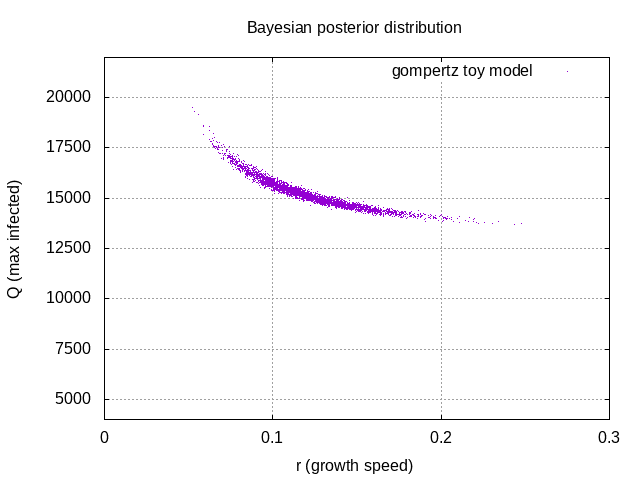
\includegraphics[width=\linewidth]{53-60-toy_gompertz.png}
    \caption{Interpolation on days 53-60.}
  \end{subfigure}
	\caption{Both the two posteriors are made of points with very small
	interpolation errors ($<2\%$), but the second one is more spread,
	i.e. contains more uncertainty,
	due to the shorter time span. The true values are
	$q = 0.05$, $Q = 20000$.}
\end{figure}


We finally remark how we did not \emph{prove} such a behavior,
but always observed it for any randomized test performed with toy-models
data, for all the models described in this manuscript.

\subsection{Cross validation}
If $\mathcal{D}^P_{1,T}$ is a dataset fulfilling the model for parameters $P$,
the same must
clearly hold for every sub-dataset of it (being then dataset just the
discrete trajectory of the ODE). In particular:

\begin{Proposition}
	Let $\mathcal{D}^P_{k, T}$ fulfill the ODE, $X^P(t)$. 
	Then this property
	holds for every sub-collection of points $\mathcal{D}^P_{k, n}$, 
	$k \leq n \leq T$.
\end{Proposition}

It means that if we have an empirical
dataset $\mathcal{D}$ and we want to perform the estimation of $P$, then
this estimation must produce the same results on every time-right-increasing
interval. Said with other words, every new day must add a coherent new data.


This trivial remark hides a pitfall: the number of days influence
the estimation performance. We are interested in remarking \emph{how}.
As already commented before, we expect to have more spread posterior
distributions for less number of days, and conversely. And we remark
again: this is not a "mistake", but rather corresponds to the fact the
with less points, a larger set of parameters $P$ is able to produce
the same small interpolation error.


For the sake of providing a clarifying picture, we attach two posterior
distributions corresponding to the same dataset obtained by a Gompertz law.
The simulation is the same as the one in the previous section.
The former interpolation uses only the first 7 days, 
the latter 35.
For larger number of days, the posterior remains essentially the same
(see e.g. figure (a) in the previous paragraph).


\begin{figure}[h!]
  \centering
  \begin{subfigure}[b]{0.4\linewidth}
    \includegraphics[width=\linewidth]{1-07-toy_gompertz.png}
    \caption{Interpolation on days 1-7.}
  \end{subfigure}
  \begin{subfigure}[b]{0.4\linewidth}
    \includegraphics[width=\linewidth]{1-35-toy_gompertz.png}
    \caption{Interpolation on days 1-35.}
  \end{subfigure}
	\caption{Both the same distributions produce points with very small
	interpolation errors ($<2\%$), but the first is more spread
	due to the shorter time span. The true values are
	$q = 0.05$, $Q = 20000$.}
  \label{fig:coffee}
\end{figure}


Summing up, in this section we understood that if $\mathcal{D}^P_{k, T}$
is a dataset fulfilling the model $X^P$, then
the posteriors corresponding to the sequence $\mathcal{D}_{k, k+n}$,
$1 \leq n \leq T$,
are initially spread, but then concentrate around stable values.
This is a property for a true ODE dataset, therefore we ask it to
be a requirement for an empirical one.
When it holds, we say that the dataset \emph{satisfies cross-validation}.


\subsection{The semigroup property}
It is realistic to think that our model might be valid
from \emph{some} day on, and not since the beginning of the dataset time.
Some (constant) parameters in a logistic map
might be connected to the average number
of daily contacts between people (as explained in section SEC).
Therefore, if a Country establishes policies
like a social lockdown, we expect their value to change and
it would be appropriate to start
a \emph{new} instance of the ODE. In other words, we can find
appropriate to split the dataset in multiple parts, each with 
its set of parameters corresponding to a "stage" of the infection's spreading.
Local newspaper give hints about turning points due to political decisions,
but we have a formal criteria to check when a new step is actually
happening.


Let $X_{X_0}^P(t)$ be our model ODE,
and $\phi_s : \mathbb{R}^n \to \mathbb{R}^n$ its associated flow,
i.e. the map $R \mapsto X_R^P(s)$
assigning initial conditions (always at time $t_0 = 0$)
to the trajectory's value at time $s$.
We point out how $s$ is fixed, so there is one flow
for each time (existence conditions are established and here not discussed).


It is known that flows enjoy the semigroup property, i.e.:
\begin{equation}
	\phi_{t + s} (X_0) = \phi_{t} ( \phi_s (X_0)) 
\end{equation}
for each initial condition $X_0$.
Therefore we deduce:
\begin{Proposition}
	If $\mathcal{D}_{k, T}$ is a dataset fulfilling $X^P$, 
	then it holds for
	$\mathcal{D}_{k+1, T}$, too.
\end{Proposition}

\begin{proof}
	By using the semigroup property, and the dataset definition
	for $\mathcal{D}_{k, T}$:
	\begin{equation}
	V_{k + i} = X_{V_k}^P(i) \quad \forall 1 \leq i \leq T
	\end{equation}
We want to prove:
	\begin{equation}
		V_{k +1 + i} = X^P_{V_{k+1}} (i) \quad \forall 1 \leq i \leq T 
	\end{equation}
But: 
\newline
	$V_{k + 1 + i} = X^P_{V_k} (i + 1)$
			[since $\mathcal{D}_{k, T}$ fulfills the ODE]
\newline
	$X^P_{V_k}(i+1) = \phi_{i + 1}(V_k)$ [flow definition]
\newline
	$\phi_{i +1}(V_k) = \phi_i \phi_1 (V_k)$ [semigroup property]
	\newline
	$\phi_i \phi_1 (V_k) = \phi_i (X^P_{V_k}(1))$ [definition of $\phi$]
	\newline
	$\phi_i (X^P_{V_k}(1)) = \phi_i(V_{k+1})$ [since 
	$X^P_{V_k}(1) = V_{k+1}$, from the dataset assumption]
	\newline
	$\phi_i(V_{k+1}) = X^P_{V_{k+1}}(i)$ [flow definition]
	\newline
	Therefor we conclude: $V_{k + 1 + i} = X^P_{V_k+1}(i)$
	as desired.
\end{proof}


Note how this property is a sort of "backward cross-validation",
specific for autonomous ODE (that's the reason for which
we insisted so much on such a choice).


If it is true that, as a concrete consequence, in theory
the estimation of $P$ must be therefore the same on every left-decreasing
dataset $\mathcal{D}^P_{k + n, T}$, the number of the
days influence on the shape of the posterior distribution precisely
as already explained in the previous sections.


Being a property of a theoretical dataset, we impose it as a requirement
on empirical datasets that we want to model.

Summing up, in this section we understood that if $\mathcal{D}^P_{k, T}$
is a dataset fulfilling $X^P$, then
the posteriors corresponding to the sequence $\mathcal{D}_{k+n, T}$,
$1 \leq n \leq T$,
are initially concentrated around stable values, 
but then become more spread due to the decreasing number of days.
When an empirical dataset satisfies such a requirement, we 
say that the \emph{semigroup property} holds.


\section {Numerical results: number of deaths}
In the previous section we 
exposed 
precise criteria that we use
to establish how reliable a numerical simulation
done by combining the bayesian interpolation
and ODE modeling is.
Summing up, every time that we have an
empirical dataset $D_{1, T}$, we then search for a $k$
such that, the data on $D_{k, T}$ produce a very small
interpolation error and satisfy both the cross-validation and the semigroup
property.


When such a $k$ is found, the model is considered to be suitable.
Then we plot the posterior distribution.
Recall that in the case of Gompertz/simple logistic, the parameter $p$
correspond to the growth's speed, while $Q$ to the asymptotic maximum.
Therefore by taking the smallest $p$ with the smallest $Q$ we
obtain the best-case scenario, while the biggest $p$, $Q$
gives us the worst-case possibility. By using these two couples,
we attach plot for predictions in the month of April. The daily increasing
rate
is also shown, simply taking the derivative of the model.


Finally, the only last element that we have not yet commented is the
intensity of the measurements error. If the numbers of observed
days is equal to $n$, then the noise $\eta$ (parameter of the Bayesian
algorithm, as explained in SEC) is chosen to be a centered gaussian
with diagonal covariance matrix $\{a_{ii}\}$, where $a_{ii}$ is equal
to the $i-th$ observed measure. In other words, each data is supposed
to have been noised with
a centered gaussian having variance equal to the final measurement itself.
This is of course an arbitrarily choice, easily replaceable.
One might argue that the error is too small or too unrealistic,
but a choice must be taken and we kept is as a starting
point.


\subsection{Number of deaths in Germany}
In this section we use logistic models as an attempt 
to predict the future number of
fatal cases in Germany. 


We take the dataset spanning from to 15th of March to the 15th of April,
and try to detect if it follows a logistic growth.

\subsubsection {Using the Gompertz law}
By applying the procedure described above, we judge the sub-dataset
going from the 25th of March to the 15th of April suitable for a Gompertz
modeling 
(therefore $k = 10$, using the notation of the previous section).
The posterior measures seem to satisfy both the cross-validation and 
the semigroup property, with an interpolation error always inferior
to $3 \%$. The values for $Q$ are always in the interval
$[6000,8000]$, while $q \in [0.07, 0.09]$.
Therefore the worst case scenario is given by the choice 
$P_1 = \{0.09, 8000\}$ (fastest growth, highest
number of deaths) and the best by $P_2 = \{0.07, 6000\}$.
The results are summed up in the following plots.

\begin{figure}[h!]
  \centering
  \begin{subfigure}[b]{0.8\linewidth}
    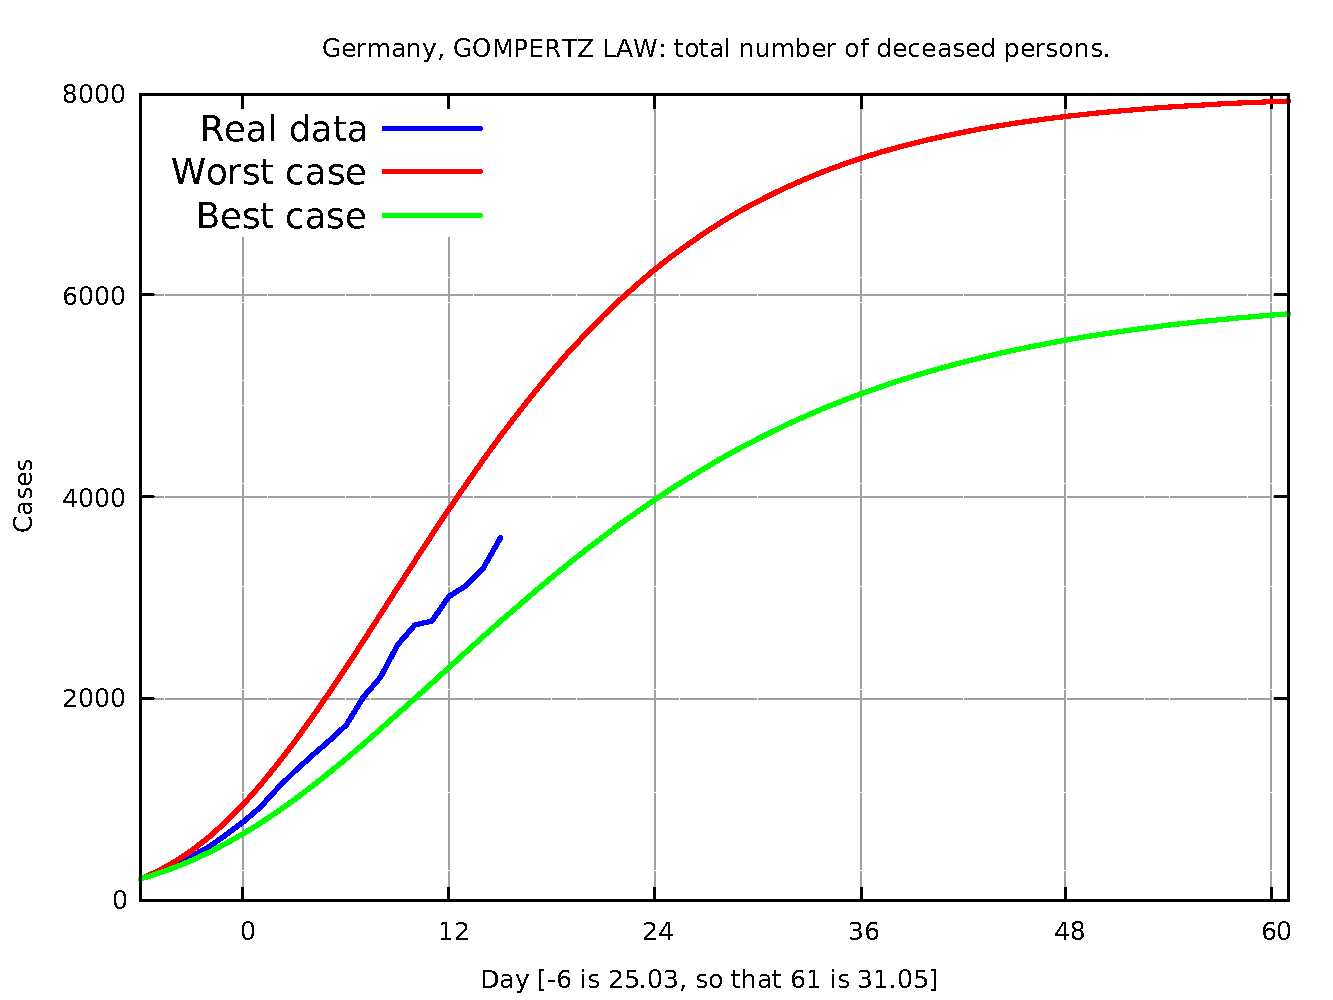
\includegraphics[width=\linewidth]{DE_g_d/DE_g_d_overview.pdf}
  \end{subfigure}
  \begin{subfigure}[b]{0.8\linewidth}
    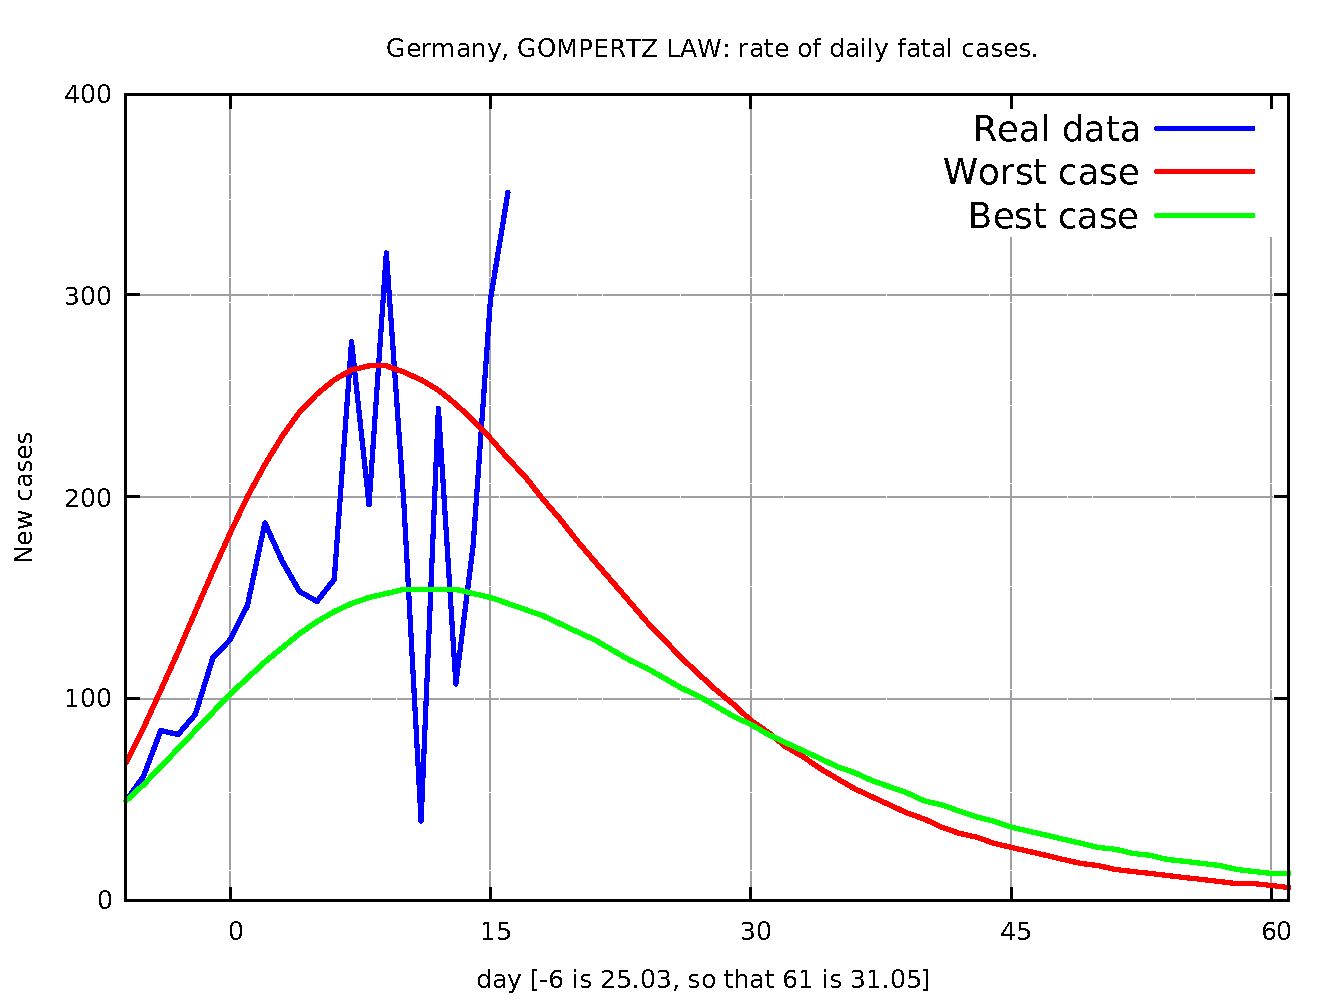
\includegraphics[width=\linewidth]{DE_g_d/DE_g_d_peak.pdf}
  \end{subfigure}
  \caption{Results by using the Gompertz law to predict the number of
	deceased people in Germany. The first plot refers to the
	\emph{total} cases, while the second to the daily increasing
	rate. The day goes from $-6$, the 25th of March (number
	of registered cases: 206), to the end of May.
	In such a way the days between 1 and 30 are precisely 
	the date in April,
	helping readability. The second plot shows how
	we surpasses the peak around the 12th of April.
	Finally, we remark clearly: 
	\textbf{according to the Gompertz model, the stable
	state is reached at the end of May}.
	It means that, assuming that the goal would be to minimize the number
	of deceased people, the actual measure should be kept constant
	until then.}
\end{figure}

\subsubsection {Using the simple Logistic law}
In the case of the simple Logistic law, we start seeing an interpolation
error always inferior than $3\%$ only after the day 13, i.e. the $15+13=28$th
of March. It was more difficult to evaluate the cross-validation and
the semigroup property of the posterior distribution, therefore we
decided delaying of some days in order to increase the possibility
of being into the lockdown stage. Therefore we chosen the
subdataset in the span 1-15th April, so $k = 18$,
but obtained a less-concentrated posterior measure.
In order to be sure of putting safe bounds,
we kept them large by registering
$Q \in [4000,5500]$ and $q \in [0.15, 0.25]$.
We recall how we do not pretend to estimate the precise number of cases, 
rather to express realistic bounds for the best and worst case scenarios.

\begin{figure}[h!]
  \centering
  \begin{subfigure}[b]{0.8\linewidth}
    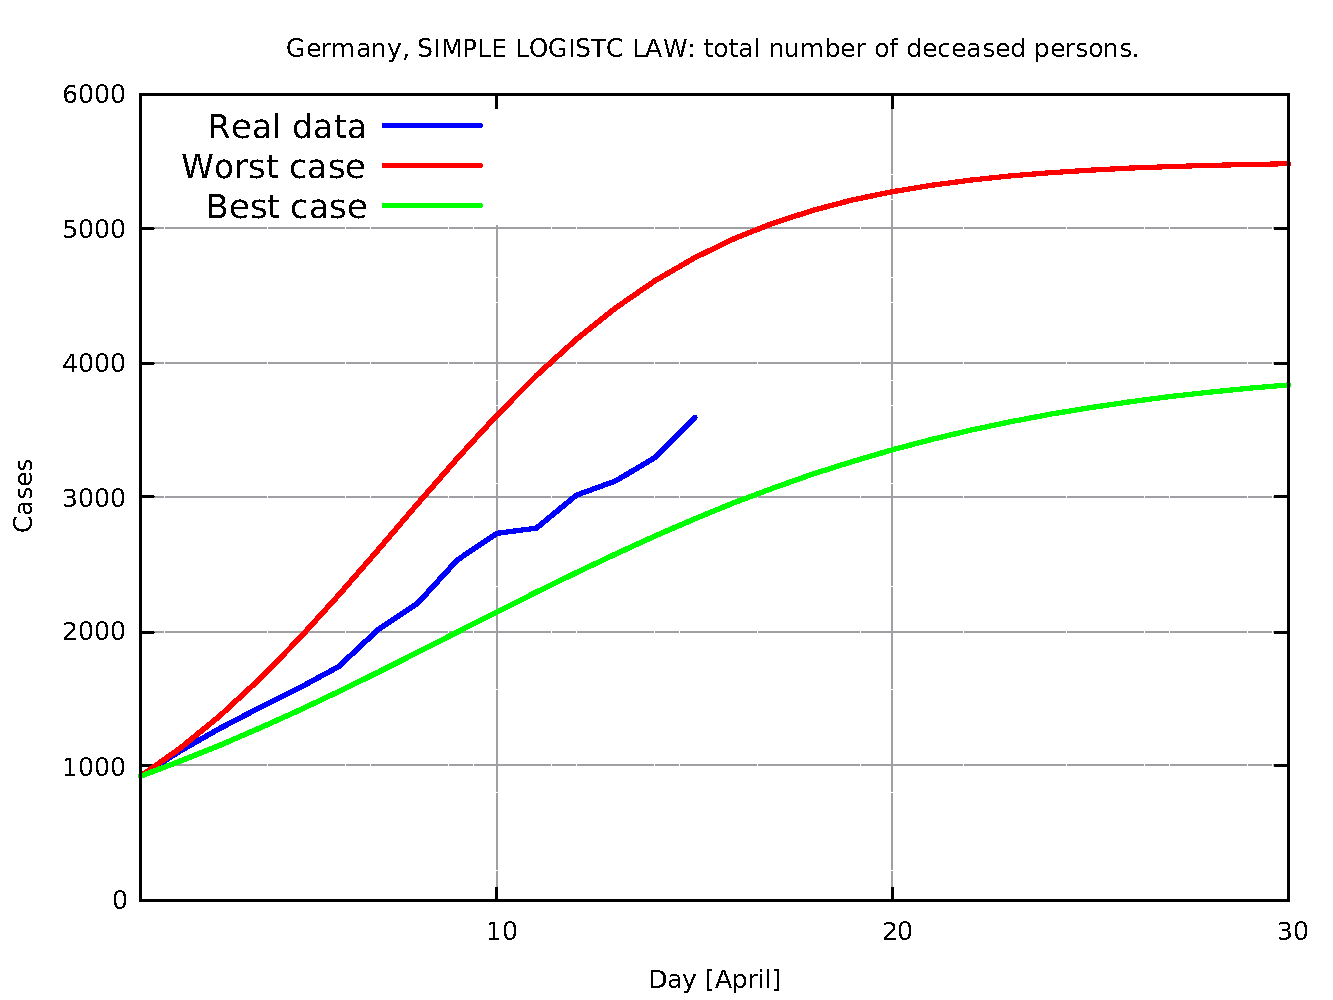
\includegraphics[width=\linewidth]{DE_l_d/DE_l_d_overview.pdf}
  \end{subfigure}
  \begin{subfigure}[b]{0.8\linewidth}
    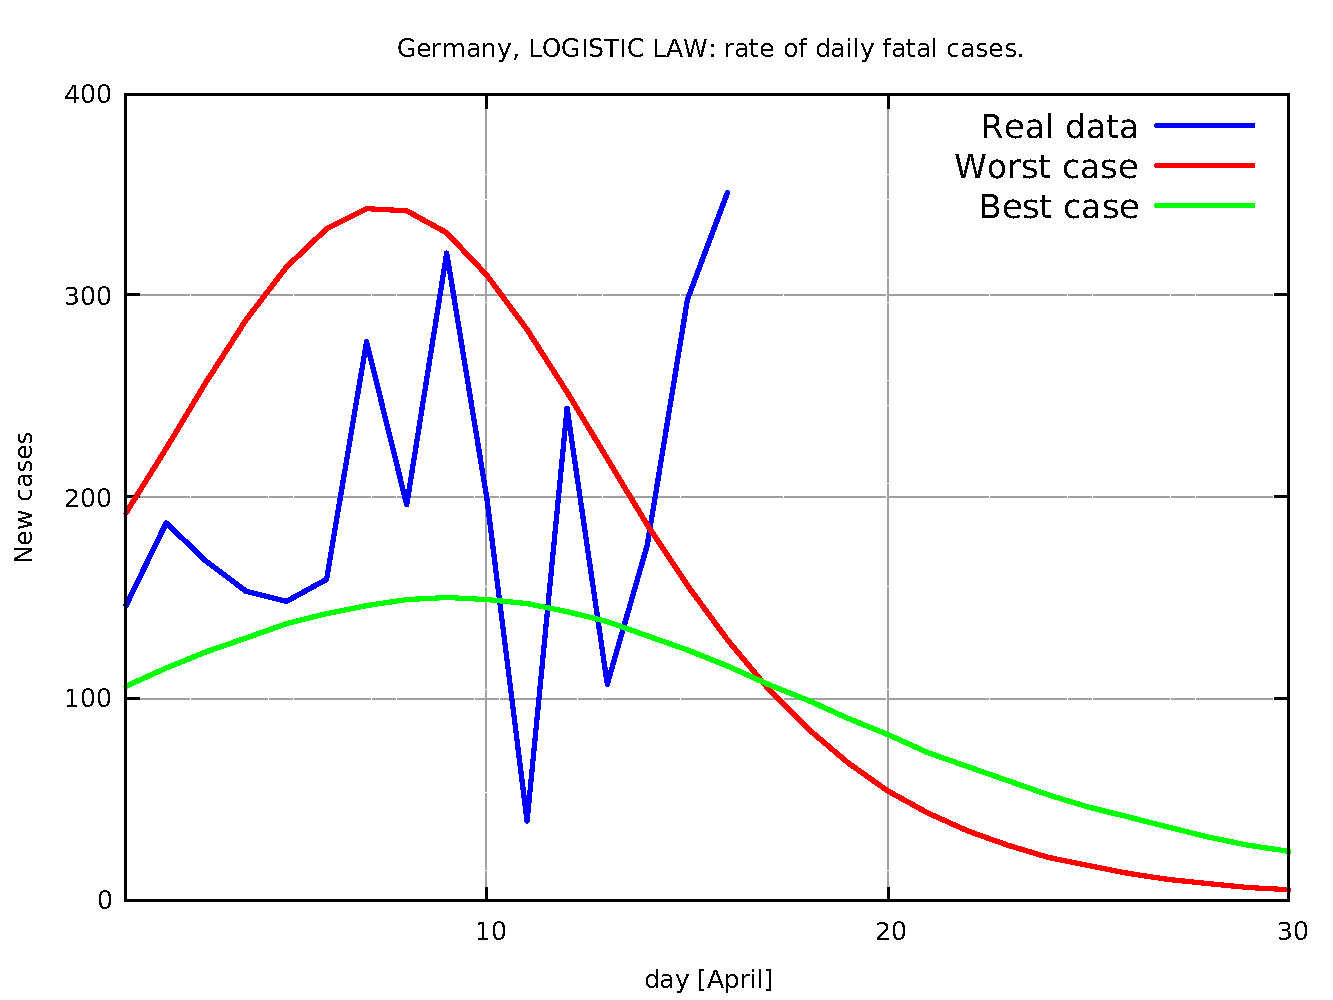
\includegraphics[width=\linewidth]{DE_l_d/DE_l_d_peak.pdf}
  \end{subfigure}
  \caption{Results by using the simple Logistic law to predict the number of
	deceased people in Germany, during the month of April.
	The first plot refers to the
	\emph{total} cases, while the second to the daily increasing
	rate.
	For this model the posterior distributions showed a possibly
	less stable behavior when compared to the Gompertz case,
	therefore we chosen larger interval of uncertainty
	to possibly prevent future oscillations.
	Although this technique, the number of daily rate
	does not sound particularly convincing.
	A remarkable qualitative behavior is that \textbf{both
	cases reaches the asymptotic maximum value at the end
	of April}, differently from Gompertz when it happened at the
	end of May. Therefore if one trusted the simple logistic map,
	can suggest to relax the lockdown measures already from the
	end of April.}
\end{figure}

\subsubsection {Using the general logistic map}
TO DO

\subsection {Number of death in Italy}
TO DO

\subsubsection{Using the Gompertz law}
TO DO

\subsubsection{Using the simple Logistic map}
TO DO

\subsubsection{Using the general Logistic map}
TO DO
\end{comment}

\section{Numerical results}

\subsection{Assumptions and methodology}
We apply the previous theory in order to formulate hypothesis 
for Italy and Germany, concerning the future number of
deceased people, whose data are considered to be more "reliable",
and the amount of total infected, information more controversial
due to test limitations and hidden asymptomatic cases.
We need to completely list and clarify the hypothesis into play,
and to explain how the results must be read.


\subsubsection{Parameters for the Bayesian technique}
In both Countries the available data start around the mid
of February, so for drawing a model 
one might be tempted to use these \emph{entire}
datasets (until today $19$th of April)
relying on the intuition "more data, more accuracy".
But in the case of logistic growths,
some parameters are connected to the average number of people's
daily contacts. Since lockdown measures have been adopted,
their values surely changed in time, resulting possibly 
in \emph{two} ODE instances: a first trajectory with the pre-lockdown
coefficients (or just possibly another model),
followed then
by a new independent one with other 
coefficients, which are the one to discover.


By considering that the countermeasures started their effects more or less 
around the $25$th of March, to increase
the chance of being in the right phase one might 
start the interpolation some days later.


But this strategy hides a pitfall: 
it's necessary to ensure that the skipped days
can actually be "forgotten" according to model under usage!
When choosing autonomous ODEs, this issue is completely solved.
Thanks to the semigroup property of the associated flow,
no matter if we start observing a value, say $V_n$, at 
day $n$, or $V_{n+1}$ at $n+1$: 
the trajectory produced from day $n+1$ (with initial
conditions $V_{n+1}$) is precisely the same of
beginning at day $n$ with initial condition $V_n$, therefore
they are ruled by the same values of $P$.


As a consequence of the reasoning above we took the safe choice
of focusing on datasets spanning from the $31$th of March to the
$19$th of April, setting so $T = 19$, and $t_i = i$, with $t_0$ 
interpreted as the $31.03$ and $t_{19}$ as the $19.04$. 


To complete the definition of the observed vector $\textbf{y}$,
we need to specify the variances $\sigma_i$ for the noises $\eta_i$.
Remarking how this is definitely an arbitrarily choice for which we do not
possess any better hint, we finally opted for setting $\sigma_i^2$
precisely as the empirical value read at day $i$. By experimenting
with data, it seemed to model a possibly "reasonable" perturbation.


Finally there is the need to fix a precise prior distribution $\rho$.
Recall that it must be
a centered Gaussian in order to use the pCN algorithm. For the general
logistic case we set the covariance matrix as
\begin{equation}
\begin{pmatrix}
	0.1^2 & 0 & 0 \\
	0 & 5000^2 & 0 \\
	0 & 0 & 0.25^2
\end{pmatrix}
\end{equation}
when working with the total number of infected,
\begin{equation}
\begin{pmatrix}
	0.1^2 & 0 & 0 \\
	0 & 3000^2 & 0 \\
	0 & 0 & 0.25^2
\end{pmatrix}
\end{equation}

when with the number of deaths.
For both the simple logistic and Gompertz laws
we used the same covariance matrix, namely the upper left 2x2 submatrix
of the general logistic above.


\subsubsection{Parameters in the pCN Algorithm}
When coming to the pCN algorithm, we set the parameter $\beta_{pcn} = 0.4$
is order to have a "compromise" between a conservative and an
exploratory Markov Chain, while the starting vector in the step $(1)$
has always chosen uniformly random. The first component, i.e.
the one referring to $q$, in $[0.01, 0.6]$, while the second ($Q$) in
$[200000,900000]$ for the infected case, $[20000,80000]$ for the
deaths in Italy and $[1000,7000]$ for the same in Germany.
When using the general logistic growth, the third component
($\nu$) started randomly in $[0.1, 3.0]$.
We set the number of samples $S_{pcn} = 5000$, and the stopping
time of the Markov Chain at $N_{pcn} = 10000$. 
The experiments run under (Slackware) Linux
using a C library for general numerical purposes developed by the authors,
and each complete simulations required between one and two
minutes on a Dell XPS 13 with a i3-8145U CPU @ 2.10GHz processor.


\subsection{Known weak points}
When using the bayesian algorithm one must carefully verify the dependence
of the results, i.e. posterior distribution $\mu$, on the choice of
the prior $\rho$. The general theoretical framework in described in REF,
but we didn't manage to check it carefully due to time constraints.
Repeating plenty of simulations on synthetic data with comparable
numbers as in the real cases,
suggested how the prior does not remarkably influence the posterior,
rather only the performance of the Monte Carlo algorithm
(e.g. more points were needed).


We are aware that structuring the noise as described 
is for sure a strong assumption,
so we tested again against toy-simulations.
For each run the true value of $P$
was therefore known, giving the possibility of computing not only the 
interpolation but also the true errors.
When setting the noise to very small values (e.g. $\sigma_i = \sigma = 0.1$)
we always obtained extremely concentrated posterior measures, with
both true and interpolation errors inferior to $1\%$. When giving the noise
larger values, the results generally kept an interpolation error
less that $3\%$, but the true errors were oscillating more, especially
in the case of the general logistic growth. This is not an error in the
algorithm, rather the fact that different parameters can give very
similar output results. When working on real data, we underline how
it does not represent a problem at all: we always consider the
\emph{whole} probabilistic distribution of parameters,
and by selecting the "most" and the "least" convenient we are able
to draw the area of uncertainty as described in the upcoming section.


Finally, we remark how the parameters for the pCN Monte Carlo algorithm
didn't seem to afflict the \emph{results}, rather only the 
\emph{performance}, and we tuned them using numerous synthetic datasets.


The convergence of the Monte Carlo algorithm was empirically checked 
by re-running with the same conditions but larger and larger stopping
times, seeing no differences in the results.


\subsection{Results}
When working with logistic models in the case of Coronavirus,
we can exploit a simple fact:
instead of the full composition of $P$,
what \emph{truly} matters is the value of 
$Q$, representing the asymptotic reached value (e.g. the maximum
number of deaths, or the maximum number of infected).
By merely plotting the posterior distribution we are able to read it.


In the case of the general logistic growth, once $Q$ is selected,
the other two parameters have generally some degree of freedom.
Conversely, when using the simple logistic or the Gompertz law,
choosing $Q$ forces automatically the parameter $q$, being the posterior
 2-dimensional.
It implies that when we plot the posterior distributions,
for these two simpler models we are able to directly get
two couple of parameters
$P_{worst}$ and $P_{best}$ corresponding to the "worst" 
(i.e. highest $Q$) and the "best" (lowest $Q$) ODE prediction.
Their are pictured two times: the first following the format
"day, number of cases", and a second 
taking into account their derivative so showing the
daily's \emph{new} cases.


Note that sometimes the posterior includes values inferior
to the current registered in real life, producing a not acceptable
result. This is not an error, rather the effect of
inserting a gaussian noise (an algorithm's mathematical requirement)
so that the measurements are equally considered
underestimated (realistic) and overestimated (not realistic). 
There is no problem with that, and it's enough to ignore these points.


We set as day zero the $31$th of March, with $774$ cases of deceased people
in Germany and $12468$ in Italy. On the same day, the number of total
infected is $71690$ in Germany and $105792$ in Italy (these are
consequently the starting conditions for all the ODEs). The time span
for the predictions  last $61$ days, 
reaching the end of May when the  asymptotic values are
always touched for all the simulated cases.

\begin{figure}[h!]
  \centering
  \begin{subfigure}[b]{0.45\linewidth}
  \includegraphics[width=\linewidth]{../de_r_d/posterior.pdf}
  \end{subfigure}
  \begin{subfigure}[b]{0.45\linewidth}
    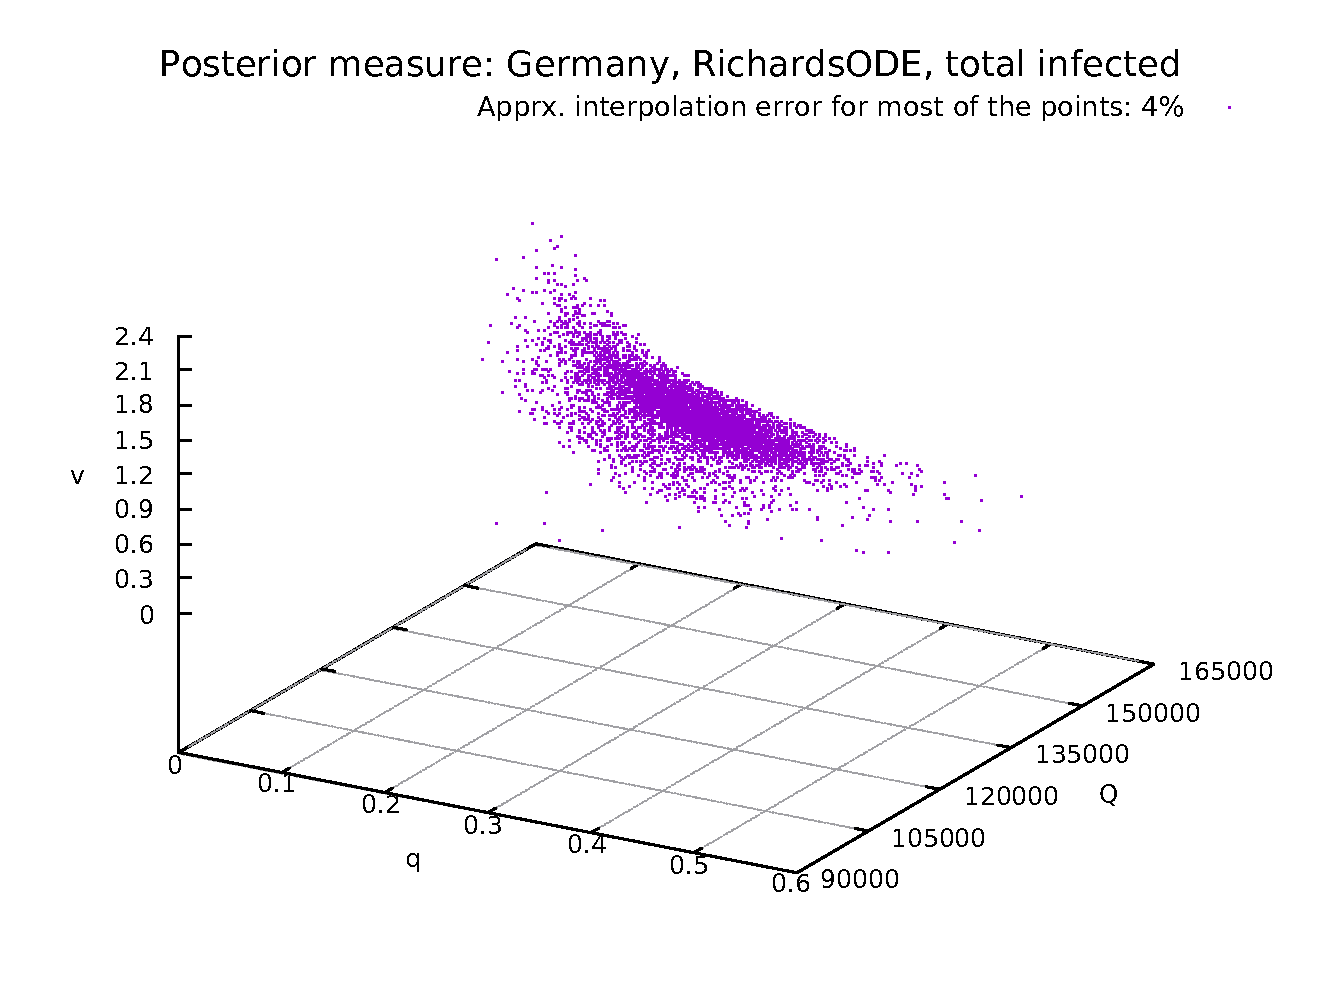
\includegraphics[width=\linewidth]{../de_r_t/posterior.pdf}
  \end{subfigure}
	\caption{Posterior distribution obtained by using the
	\textbf{general logistic} growth models on \textbf{Germany}. 
	The number of \textbf{deaths}
	and the number of total \textbf{infected} are taken into analysis.
	The former is bounded between $5500$ and
	$9000$, while the latter surely below $170000$. The \emph{same}
	results are then obtained with the Gompertz and simple logistic map,
	but there it's easier to also understand the growth's rate.}	
\end{figure}

\begin{figure}[h!]
  \centering
  \begin{subfigure}[b]{0.48\linewidth}
  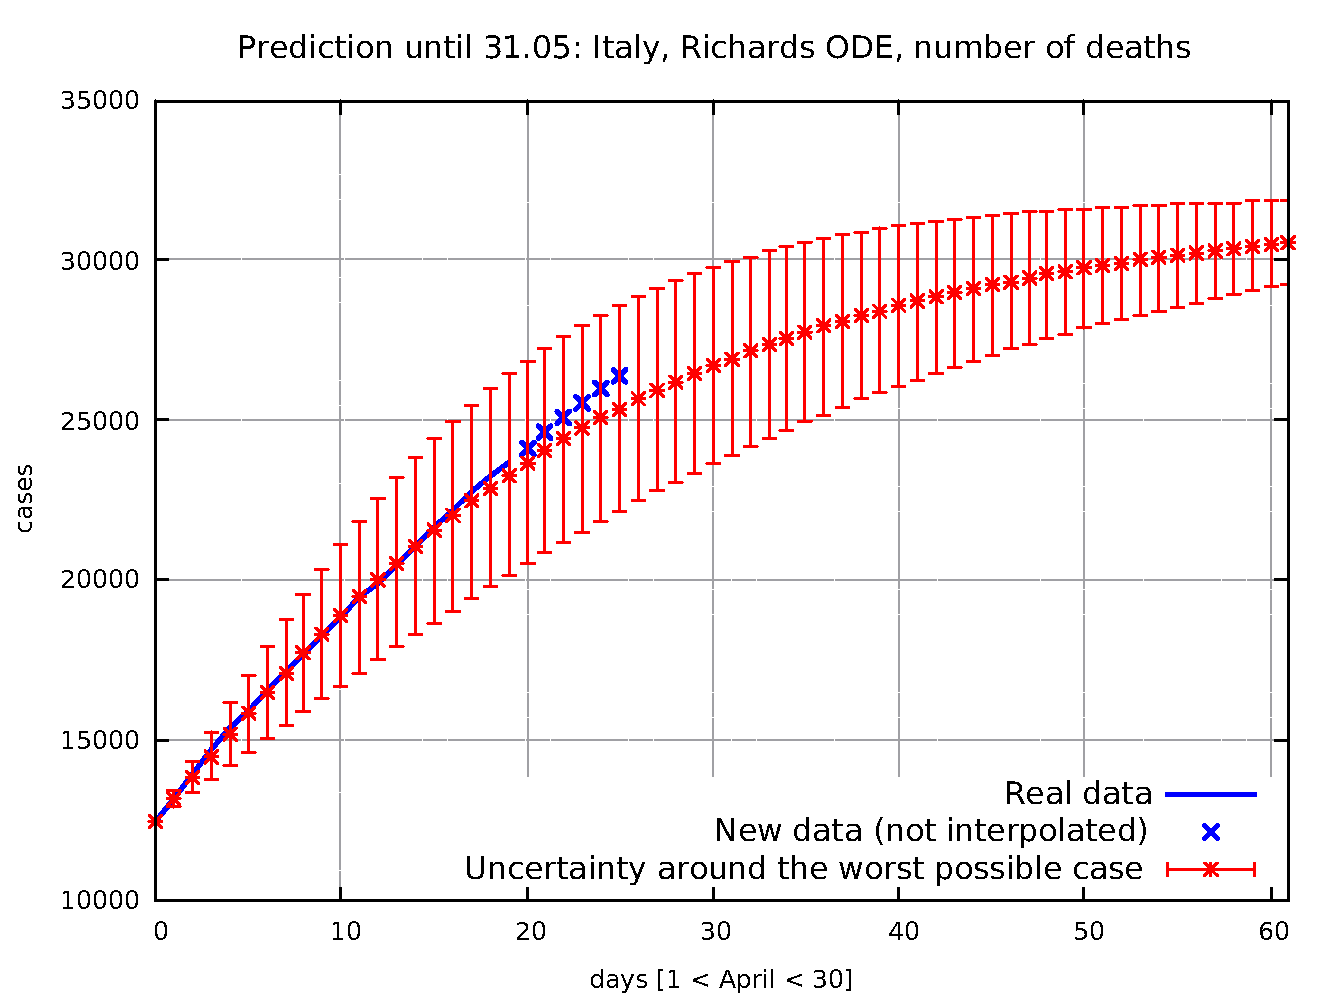
\includegraphics[width=\linewidth]{../de_r_d/prediction.pdf}
  \end{subfigure}
  \begin{subfigure}[b]{0.48\linewidth}
    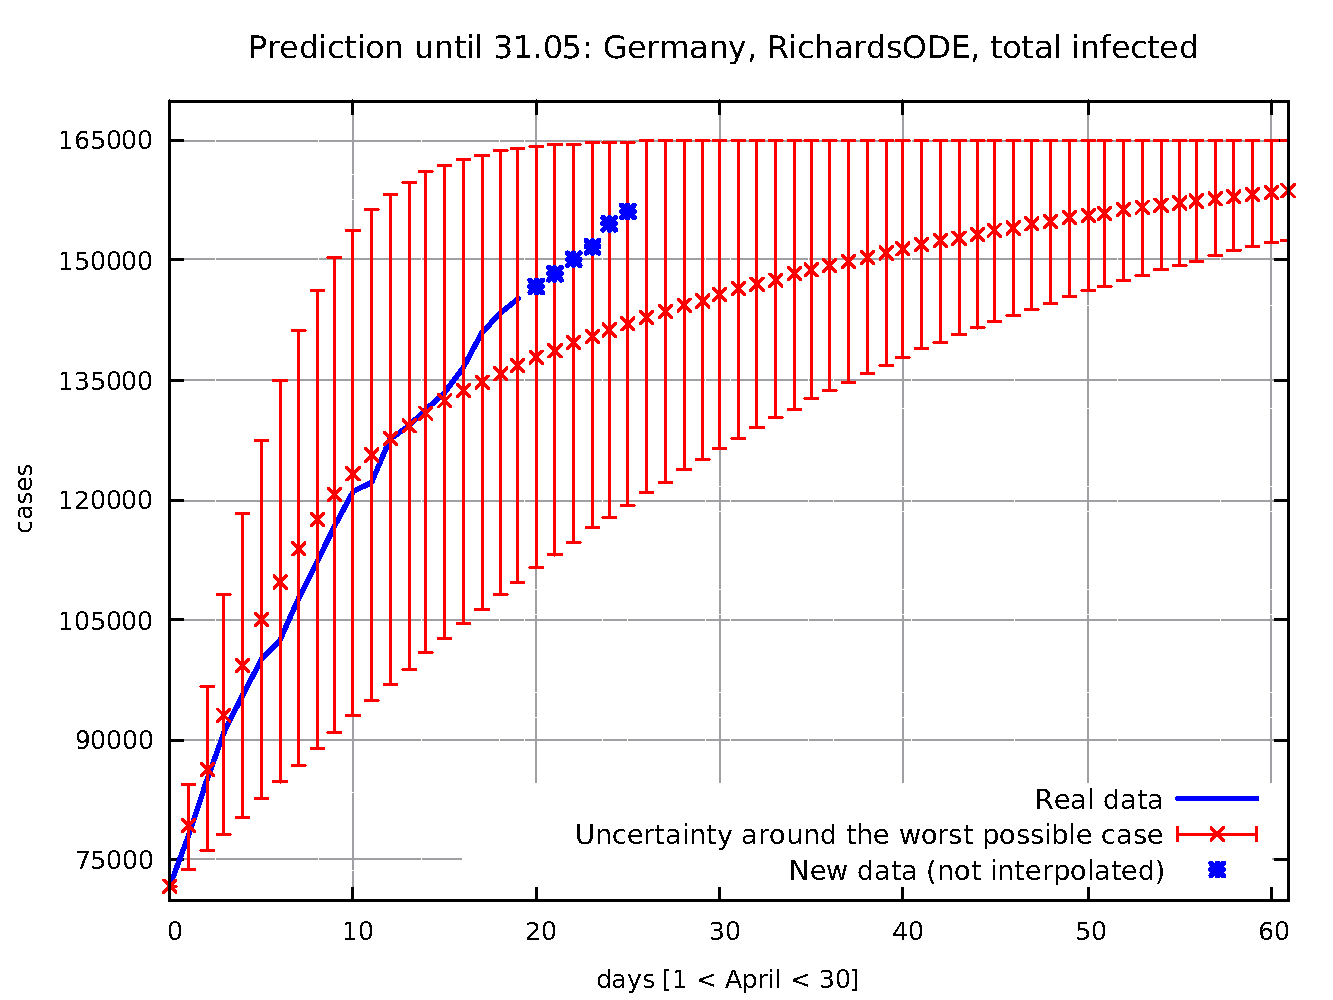
\includegraphics[width=\linewidth]{../de_r_t/prediction.pdf}
  \end{subfigure}
	\caption{to write}
\end{figure}


\begin{figure}[h!]
  \centering
  \begin{subfigure}[b]{0.48\linewidth}
  \includegraphics[width=\linewidth]{../it_r_d/posterior.pdf}
  \end{subfigure}
  \begin{subfigure}[b]{0.48\linewidth}
    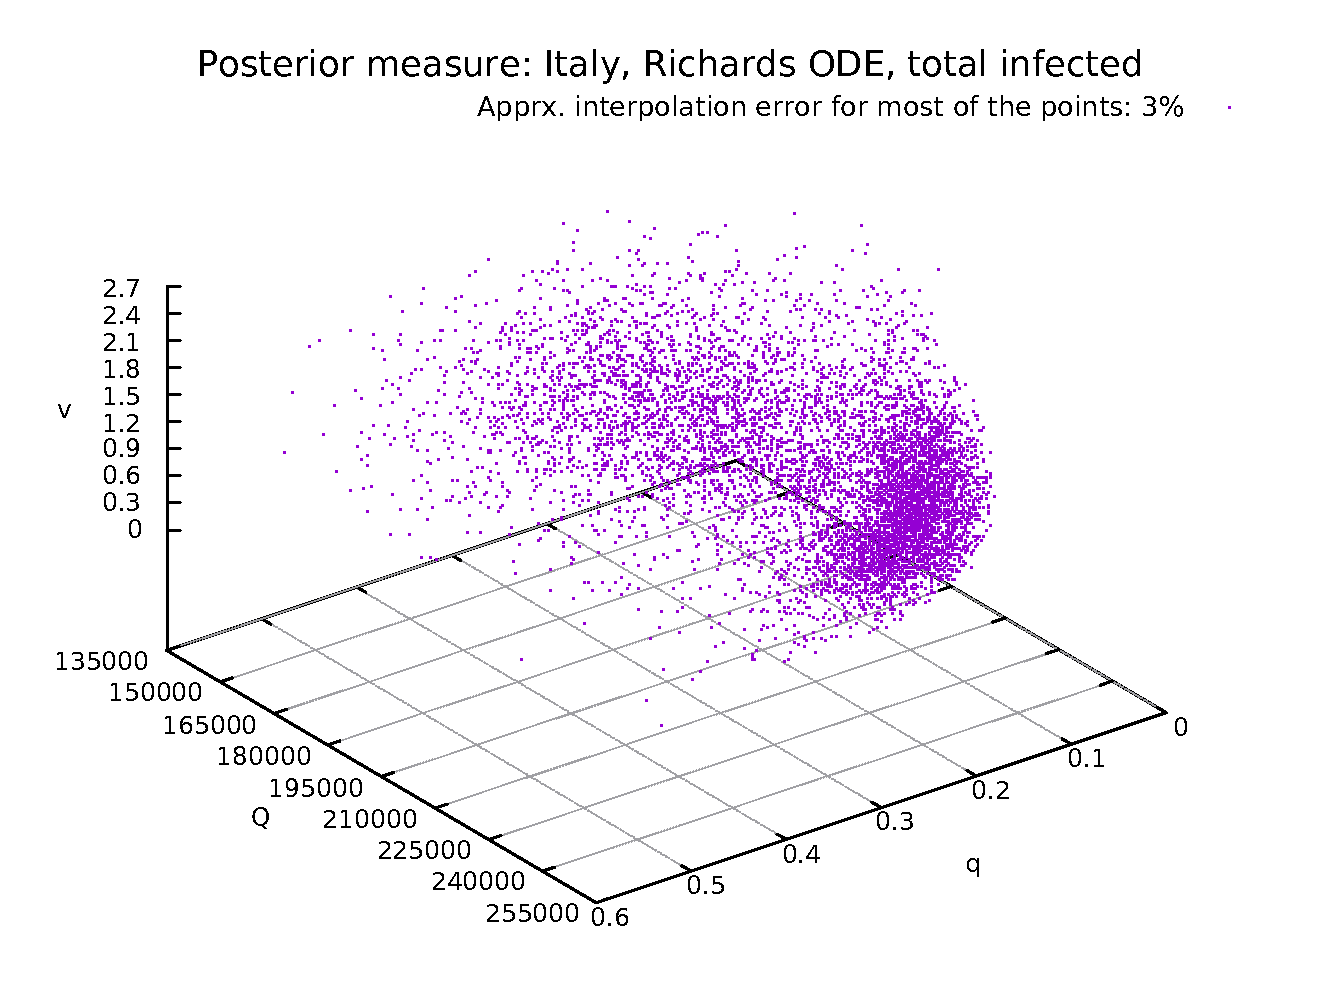
\includegraphics[width=\linewidth]{../it_r_t/posterior.pdf}
  \end{subfigure}
	\caption{Posterior distribution obtained by using the
	\textbf{general logistic} growth models on \textbf{Italy}. 
	The number of \textbf{deaths}
	and the number of total \textbf{infected} are taken into analysis.
	The former is bounded between $27000$ and
	$34000$, the latter stays below $250000$. The \emph{same}
	results will be obtained with the Gompertz and simple logistic map,
	where it's easier to estimate the growth's rate.}
\end{figure}


\begin{figure}[h!]
  \centering
  \begin{subfigure}[b]{0.5\linewidth}
  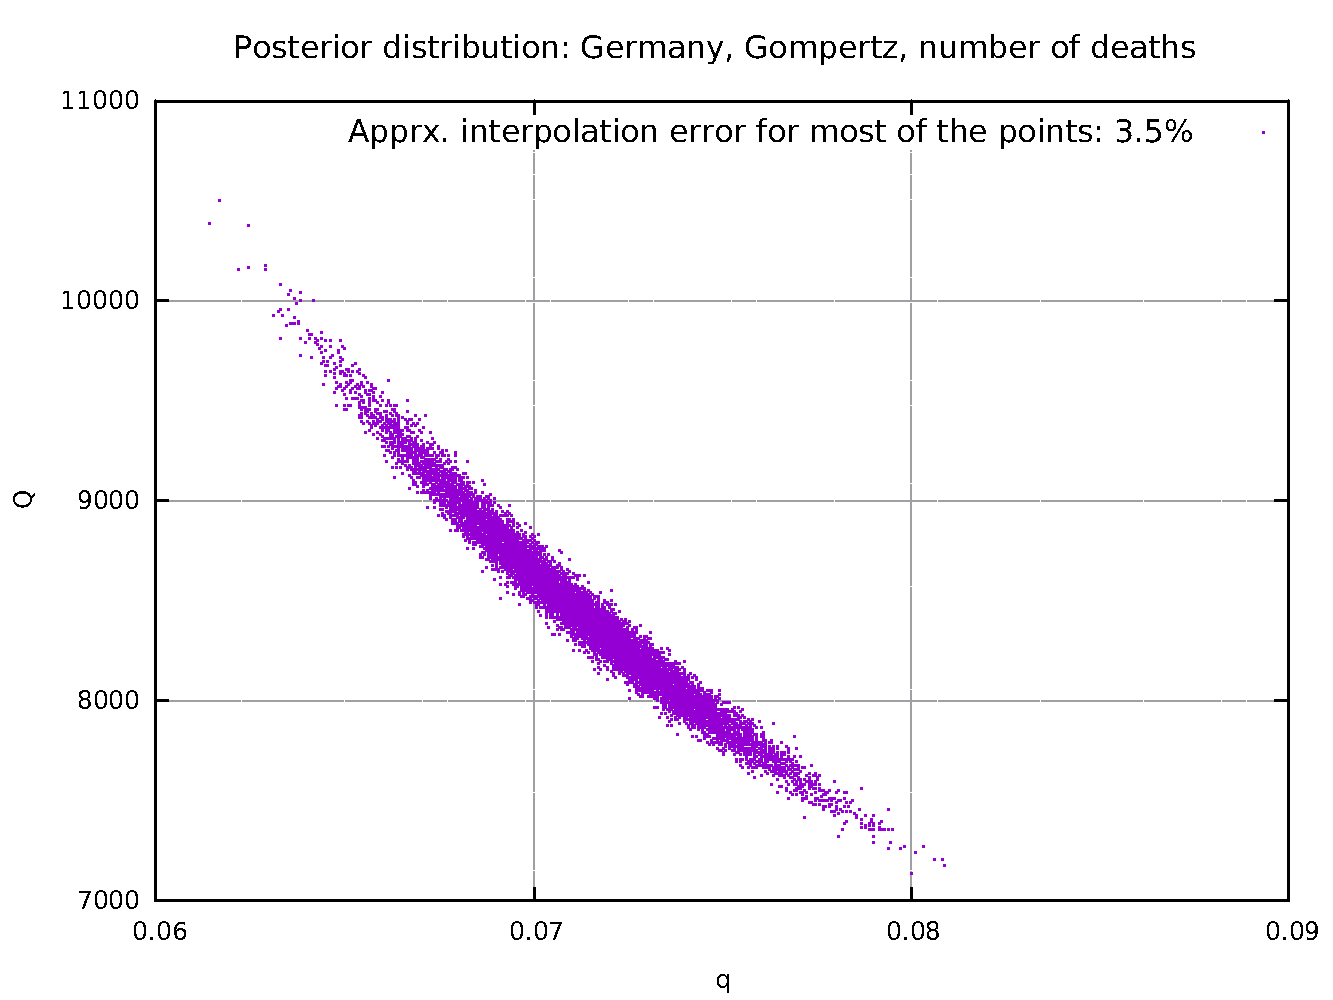
\includegraphics[width=\linewidth]{../de_g_d/posterior.pdf}
  \end{subfigure}
  \begin{subfigure}[b]{0.48\linewidth}
    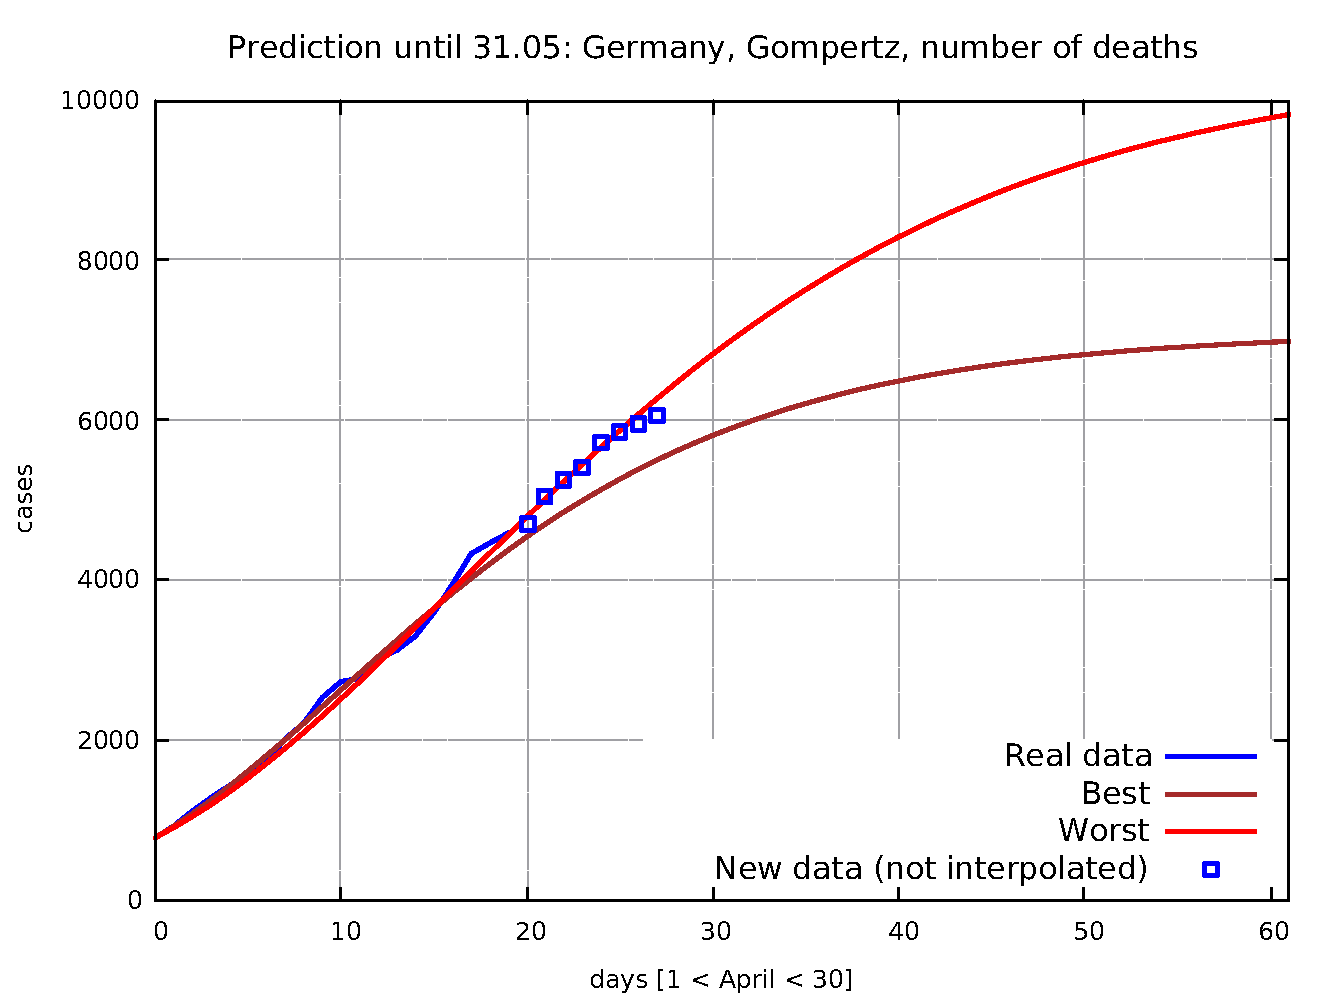
\includegraphics[width=\linewidth]{../de_g_d/prediction.pdf}
  \end{subfigure}
  \begin{subfigure}[b]{0.48\linewidth}
  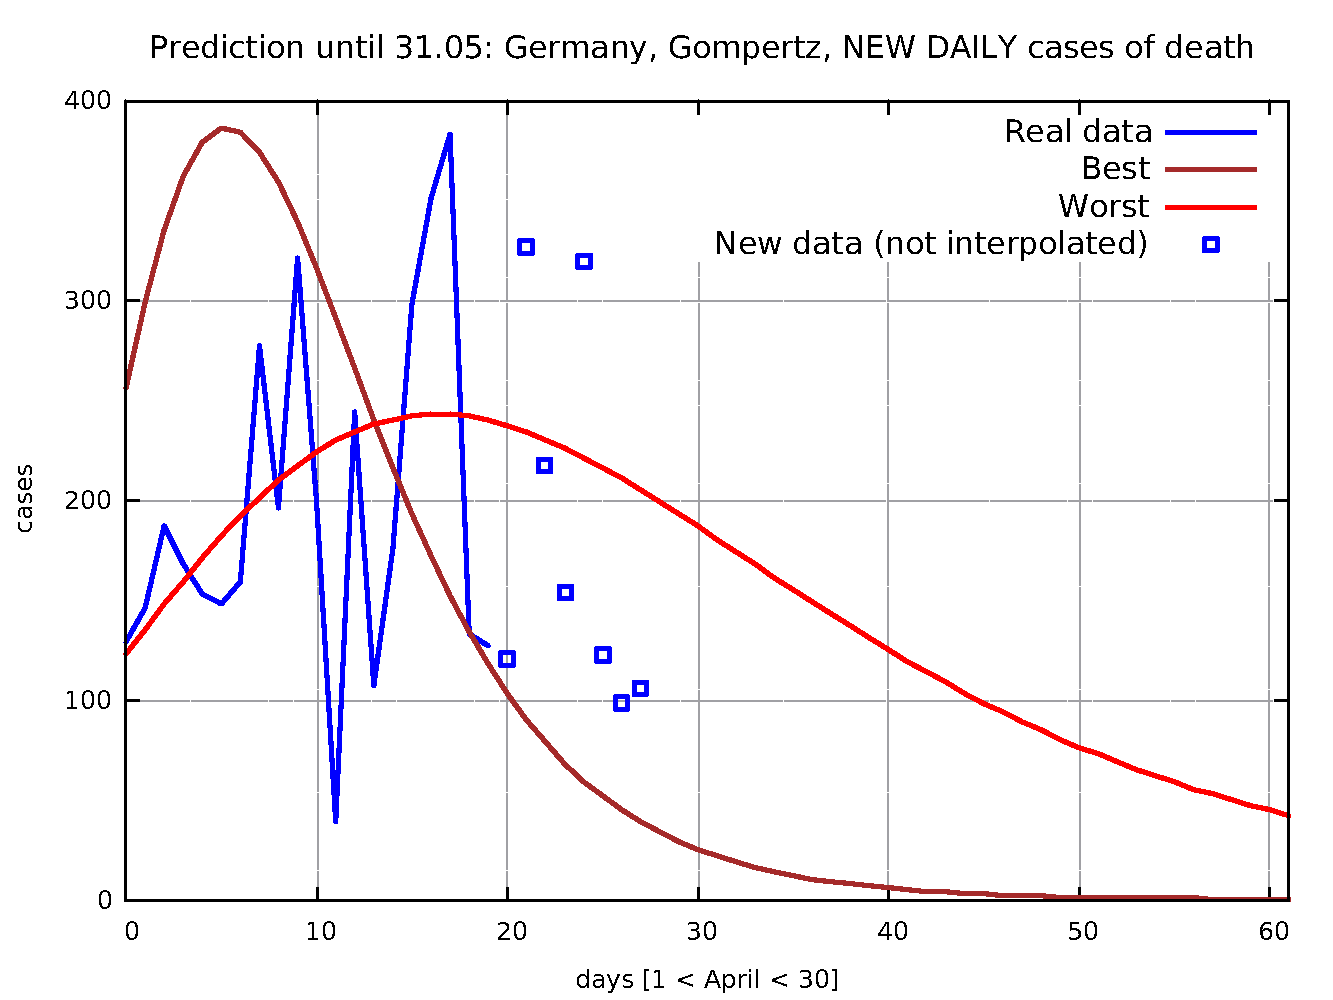
\includegraphics[width=\linewidth]{../de_g_d/peak/peak_prediction.pdf}
  \end{subfigure}
	\caption{Predicting the number of \textbf{deceased}
	people in \textbf{Germany} until the
	end of May. Result according to the 
	\textbf{Gompertz} model, which produced
	an interpolation error of around $3\%$.}
\end{figure}


\begin{figure}[h!]
  \centering
  \begin{subfigure}[b]{0.5\linewidth}
  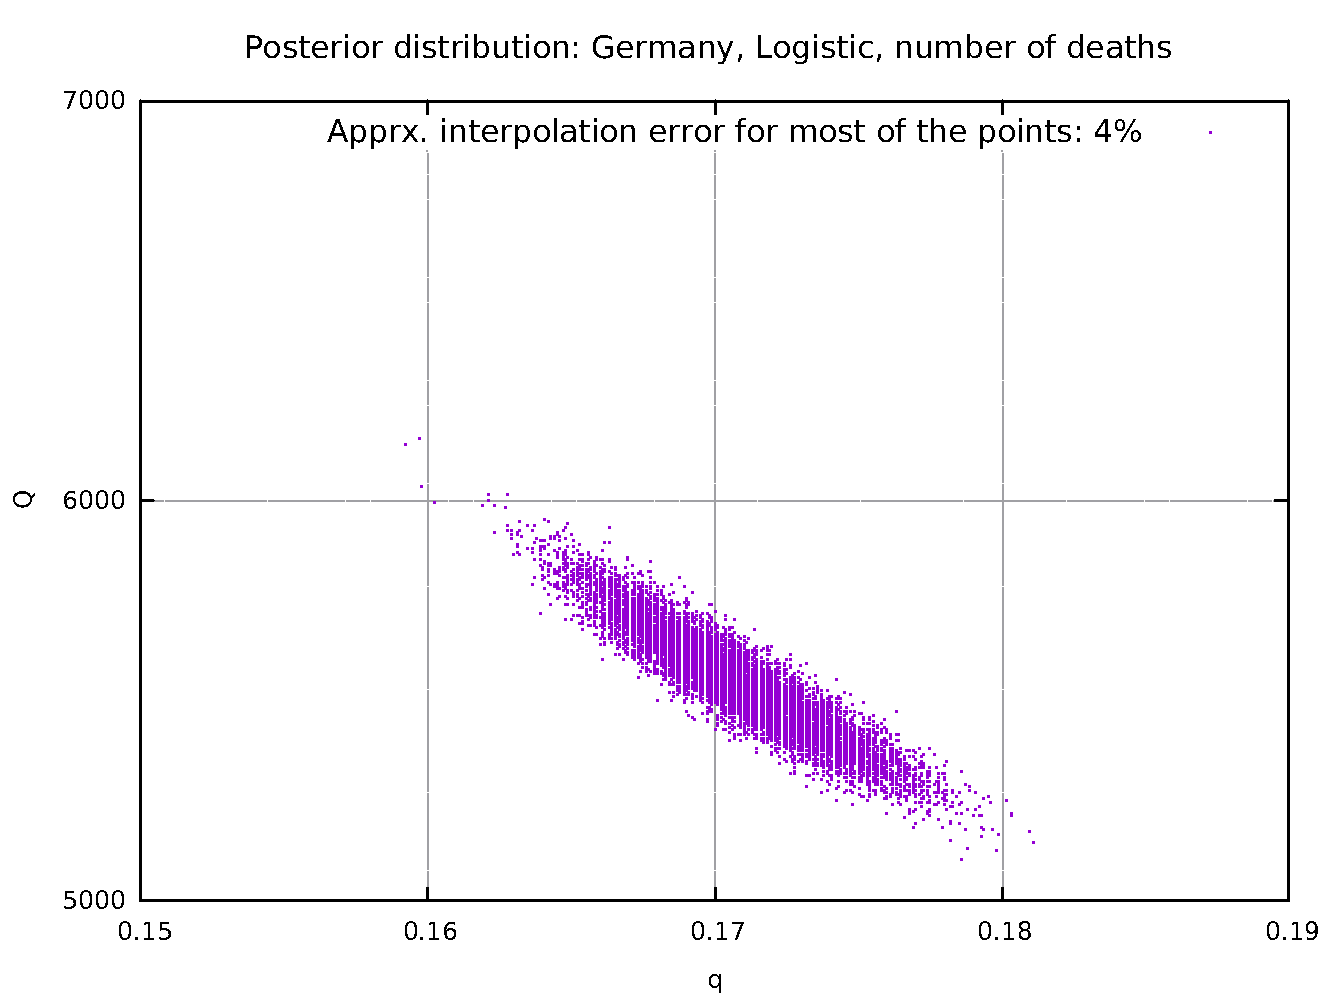
\includegraphics[width=\linewidth]{../de_l_d/posterior.pdf}
  \end{subfigure}  
	\begin{subfigure}[b]{0.48\linewidth}
    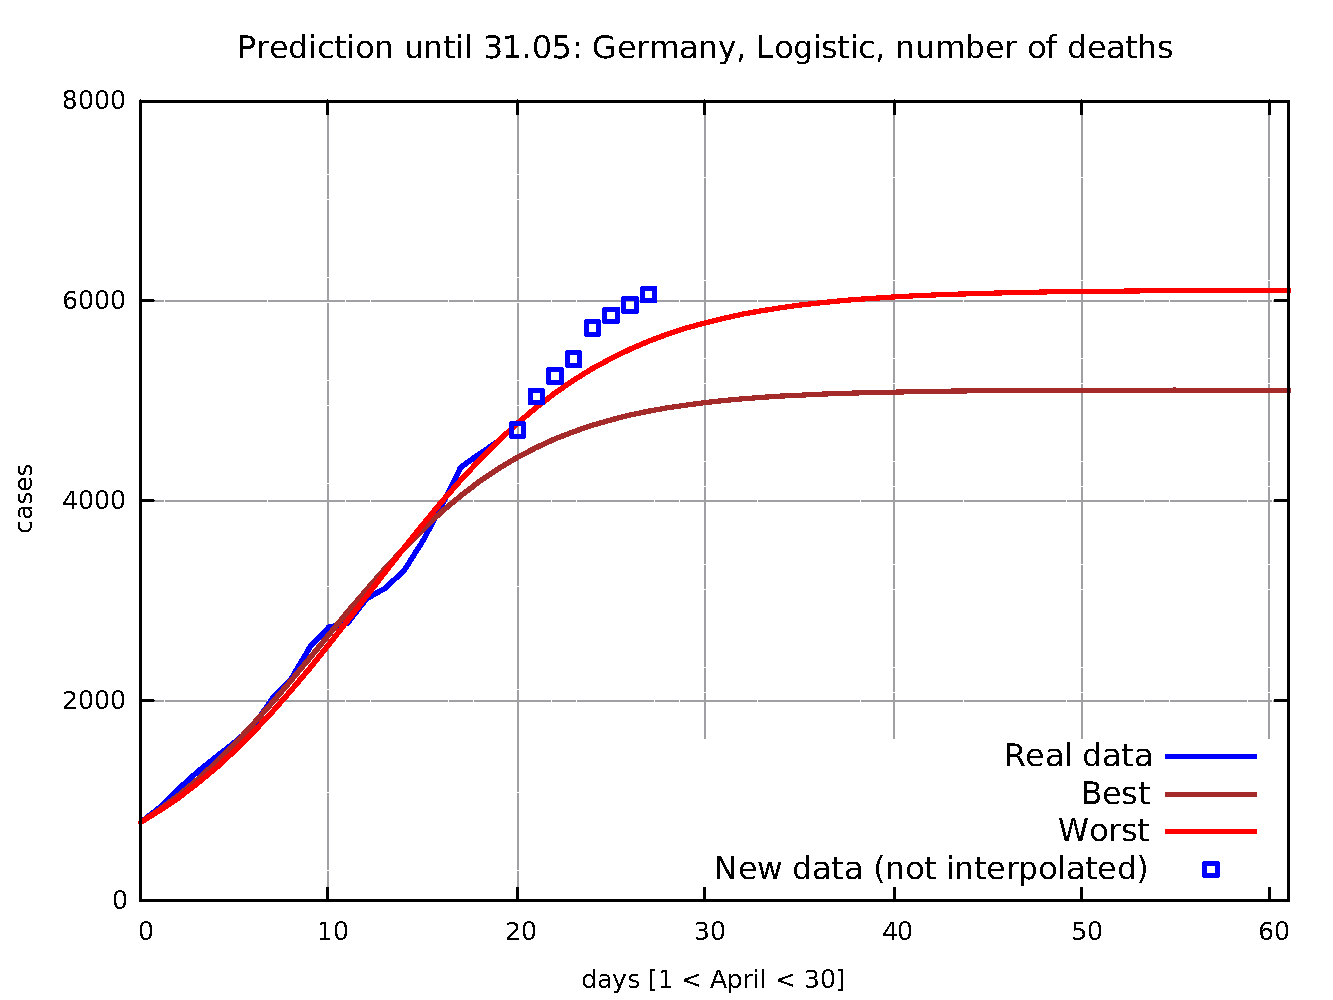
\includegraphics[width=\linewidth]{../de_l_d/prediction.pdf}
  \end{subfigure}
  \begin{subfigure}[b]{0.48\linewidth}
  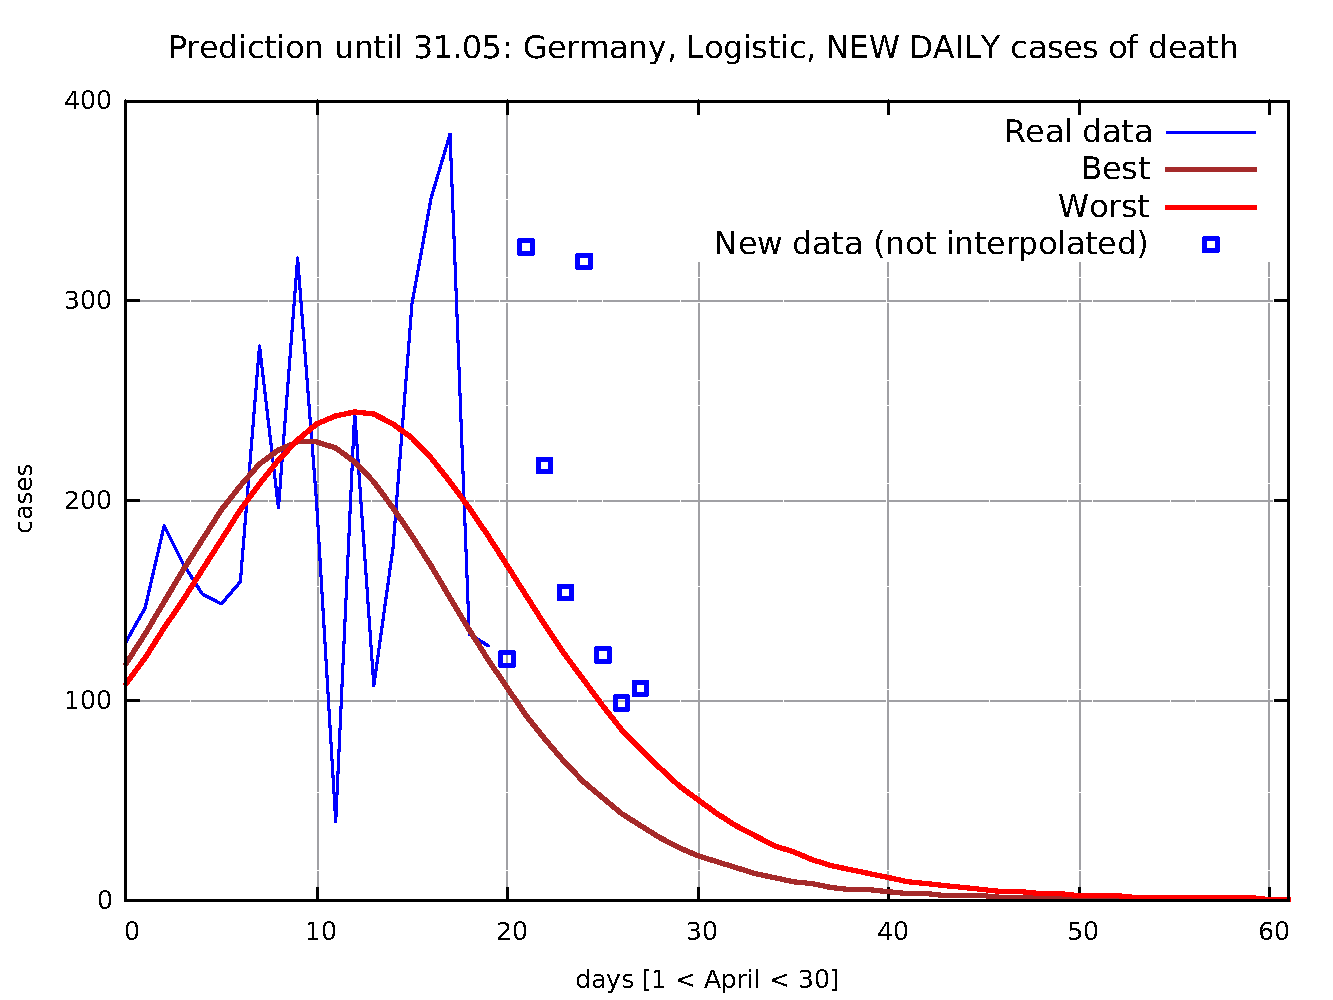
\includegraphics[width=\linewidth]{../de_l_d/peak/peak_prediction.pdf}
  \end{subfigure}
	\caption{Predicting the number of \textbf{deceased}
	people in \textbf{Germany} until the
	end of May. Result according to the \textbf{simple logistic} map, 
	interpolation error around $4\%$.}
\end{figure}


\begin{figure}[h!]
  \centering
  \begin{subfigure}[b]{0.5\linewidth}
  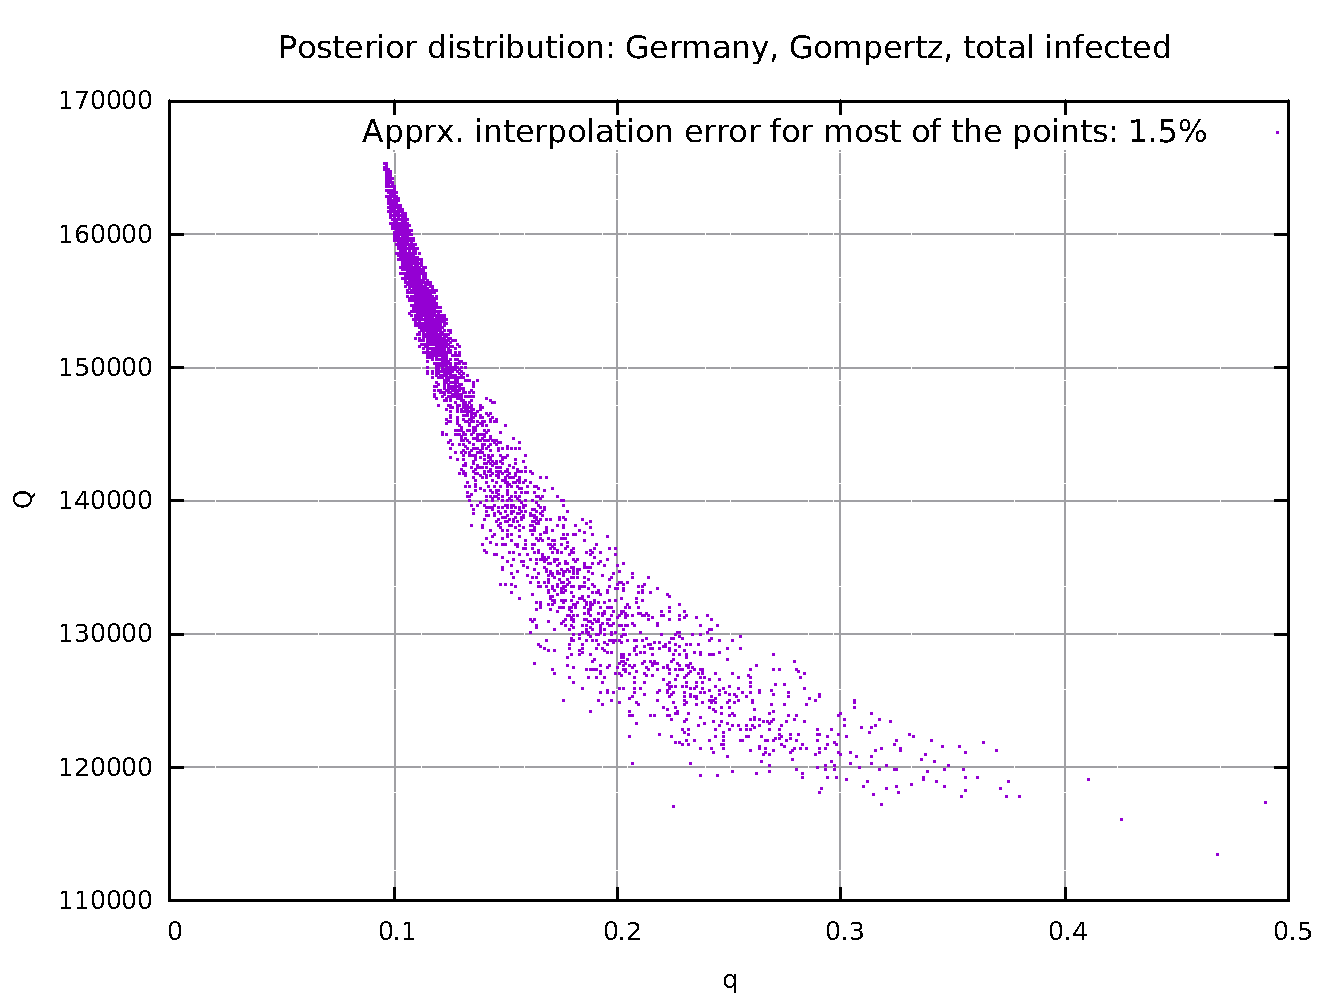
\includegraphics[width=\linewidth]{../de_g_t/posterior.pdf}
  \end{subfigure}
  \begin{subfigure}[b]{0.48\linewidth}
    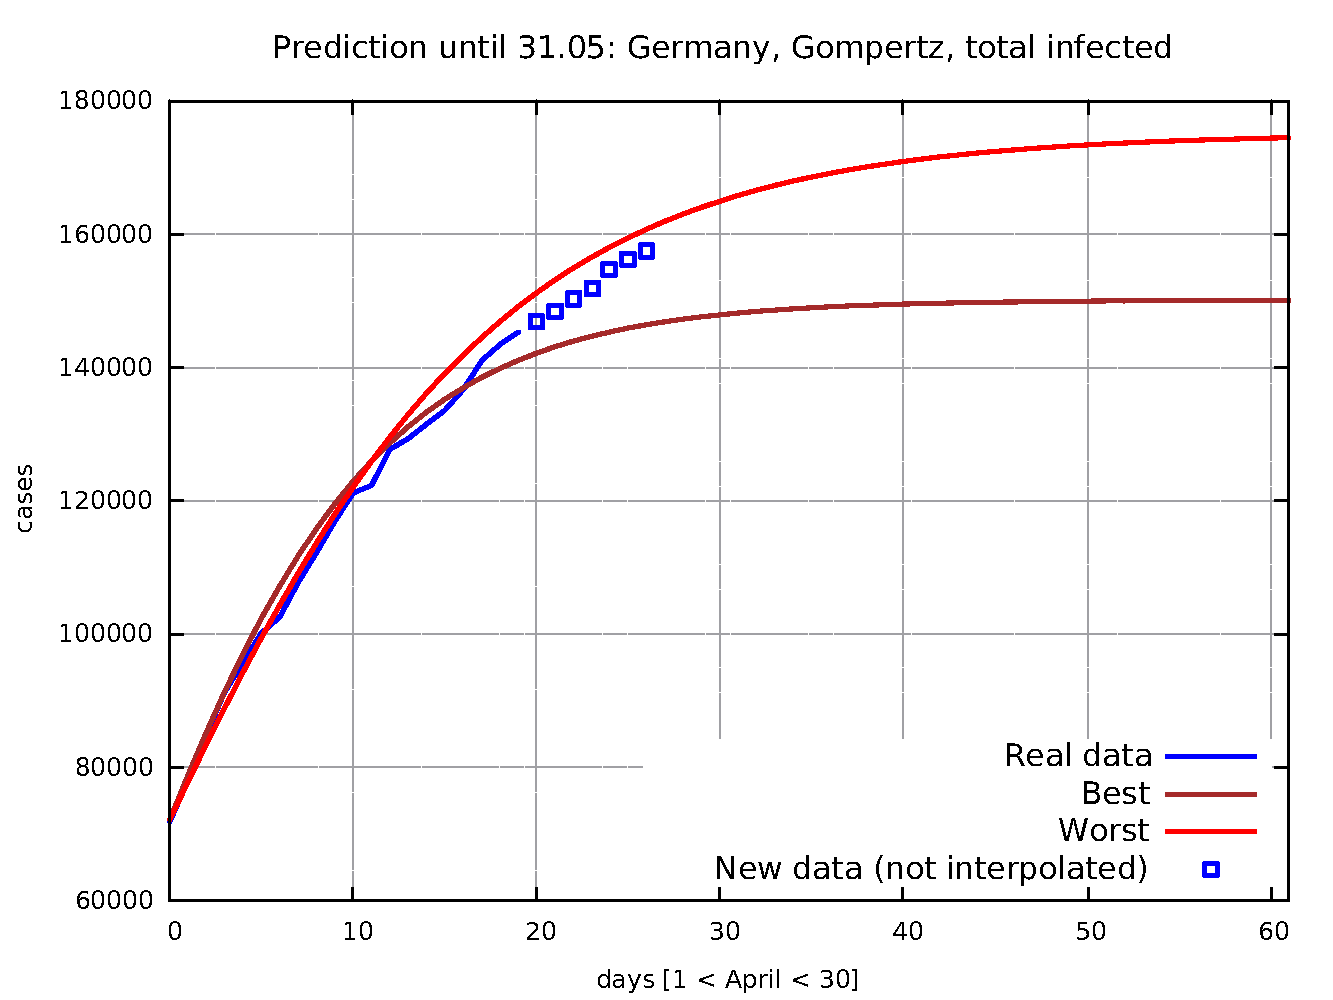
\includegraphics[width=\linewidth]{../de_g_t/prediction.pdf}
  \end{subfigure}
  \begin{subfigure}[b]{0.48\linewidth}
  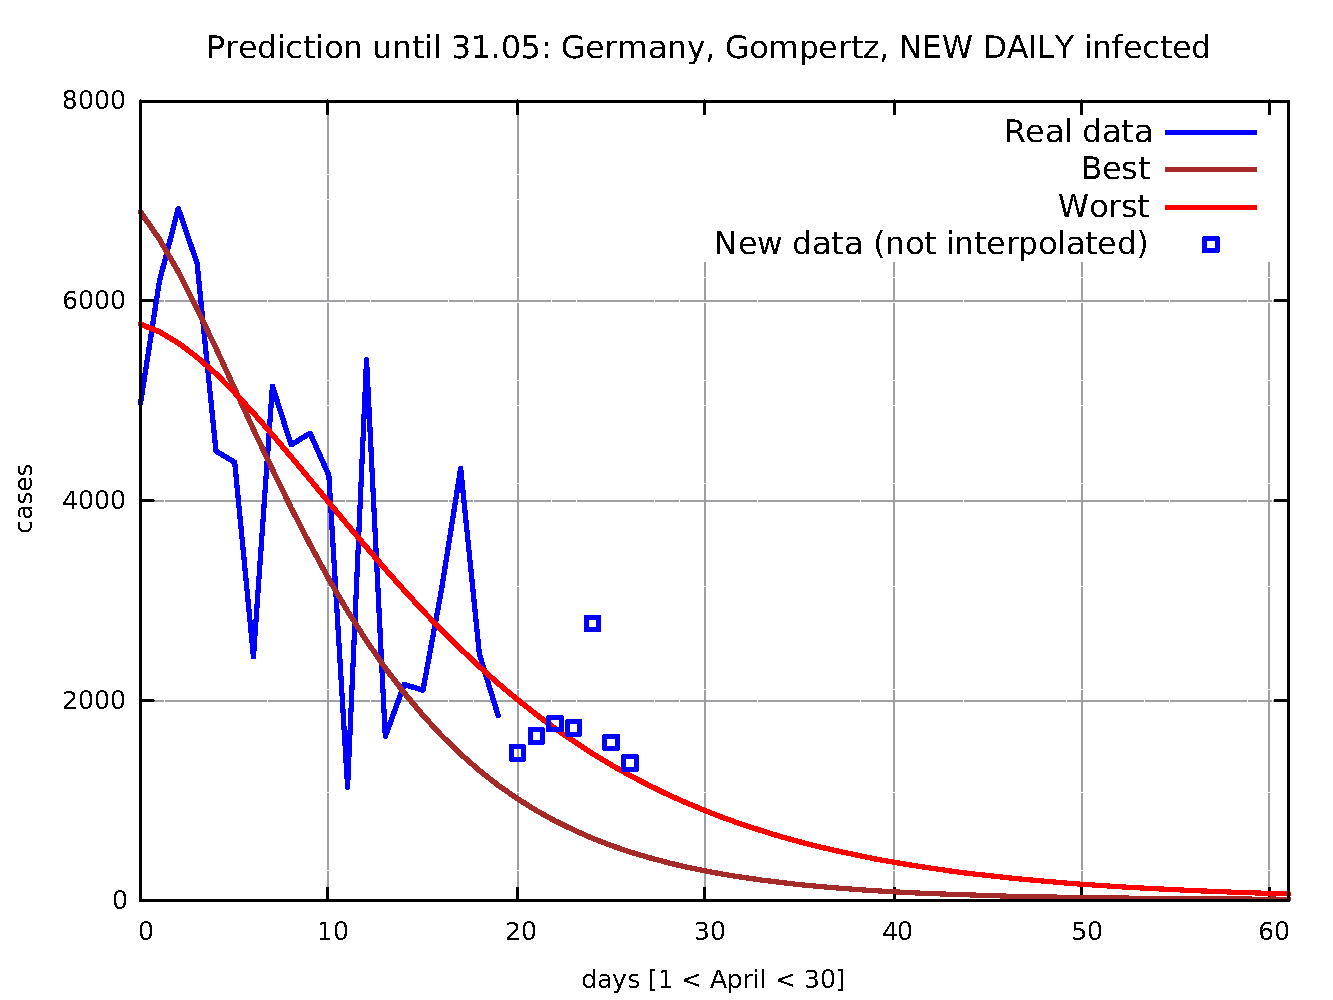
\includegraphics[width=\linewidth]{../de_g_t/peak/peak_prediction.pdf}
  \end{subfigure}
	\caption{Predicting the number of the total \textbf{infected}
	people in \textbf{Germany}
	before the end of May. Results according to the 
	\textbf{Gompertz}
	law; interpolation error of $1.5\%$.}
\end{figure}


\begin{figure}[h!]
  \centering
  \begin{subfigure}[b]{0.5\linewidth}
  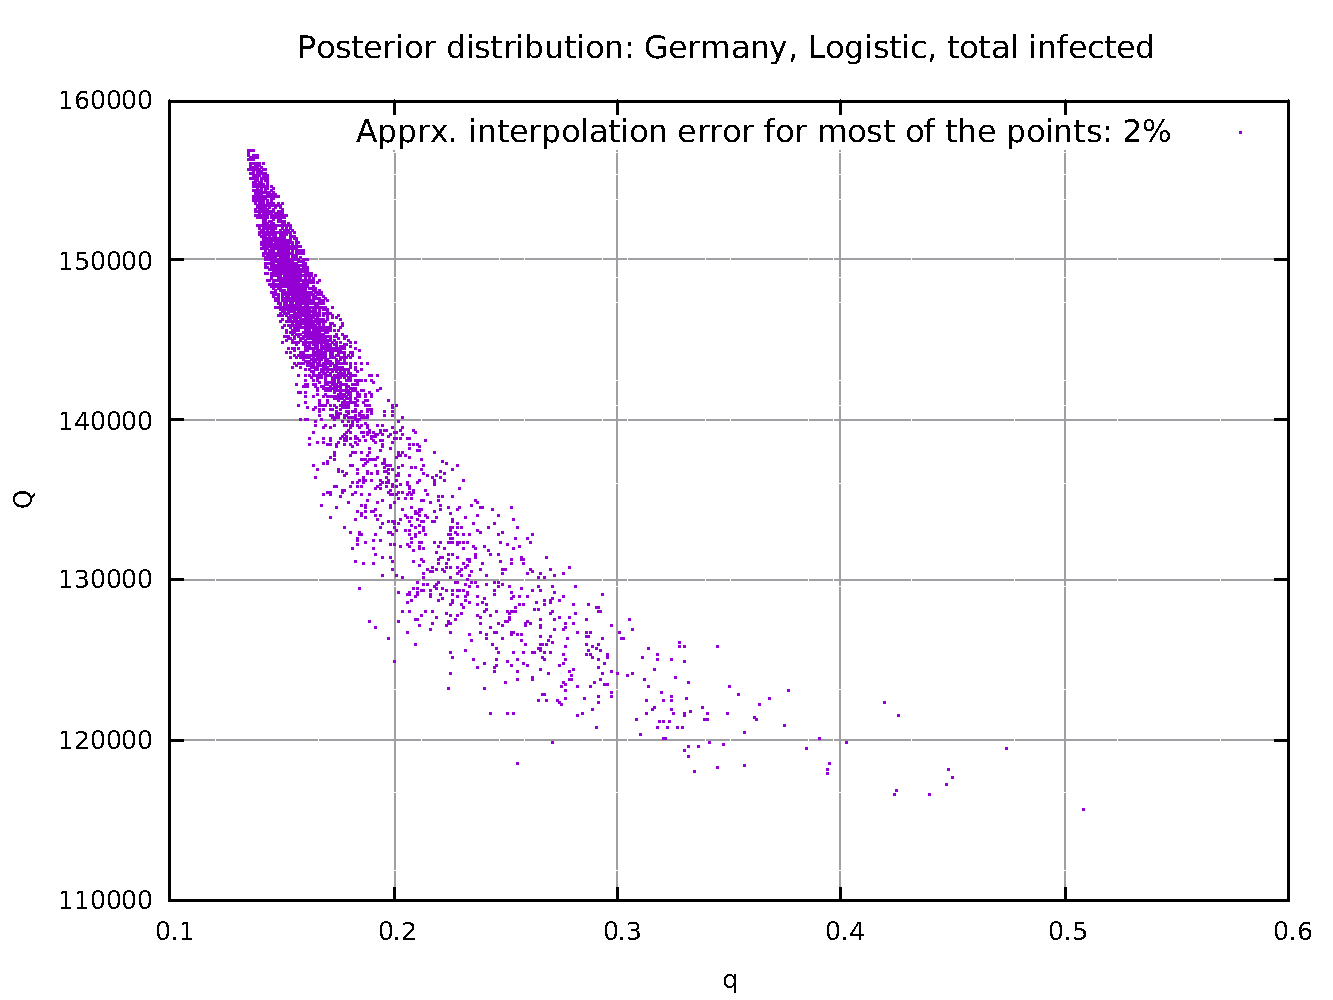
\includegraphics[width=\linewidth]{../de_l_t/posterior.pdf}
  \end{subfigure}  \begin{subfigure}[b]{0.48\linewidth}
    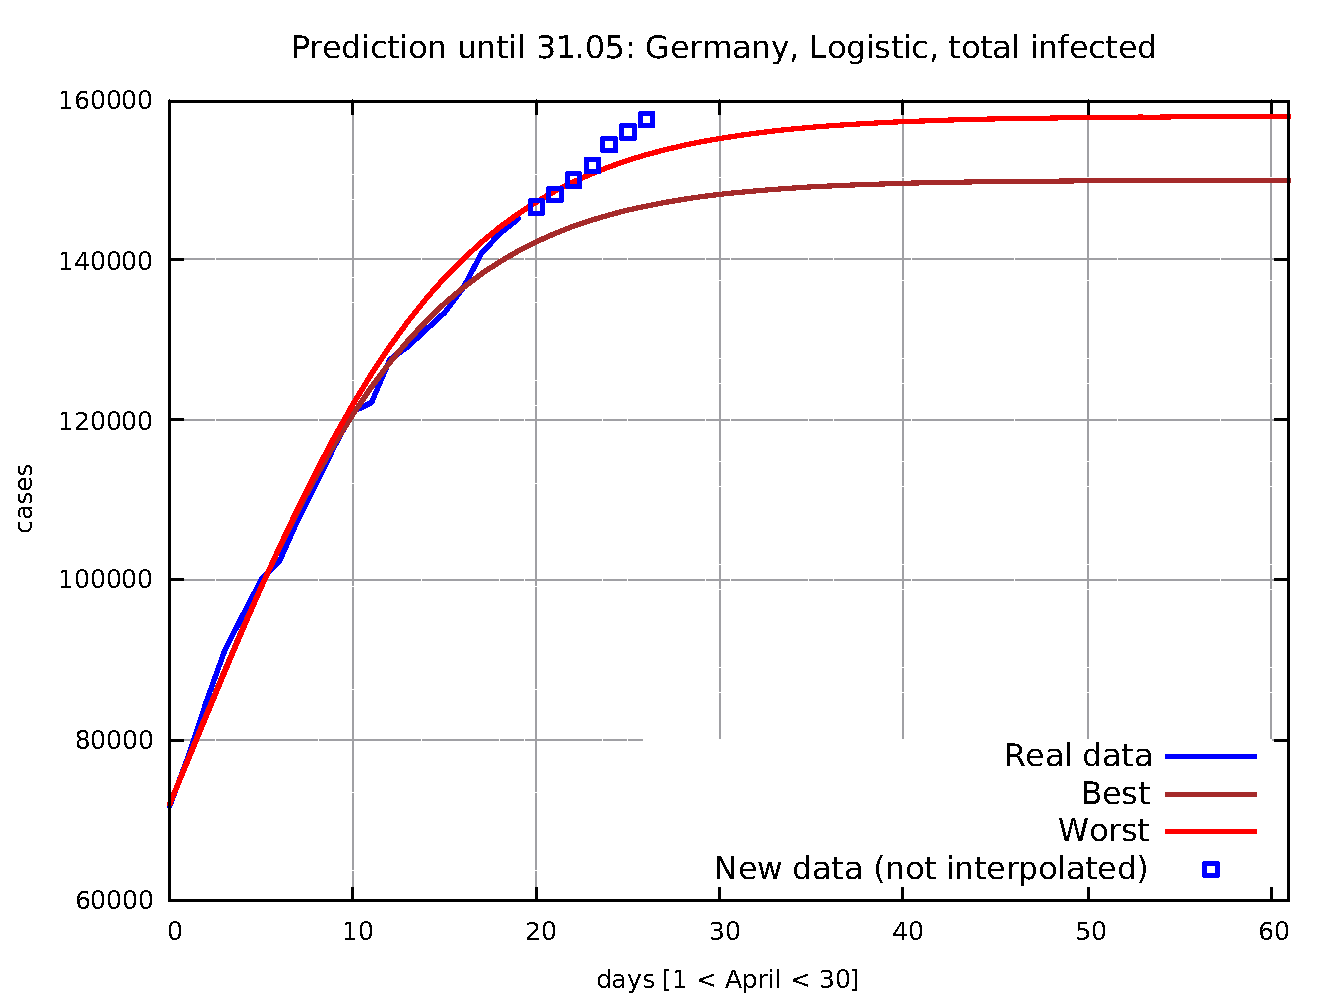
\includegraphics[width=\linewidth]{../de_l_t/prediction.pdf}
  \end{subfigure}
  \begin{subfigure}[b]{0.48\linewidth}
  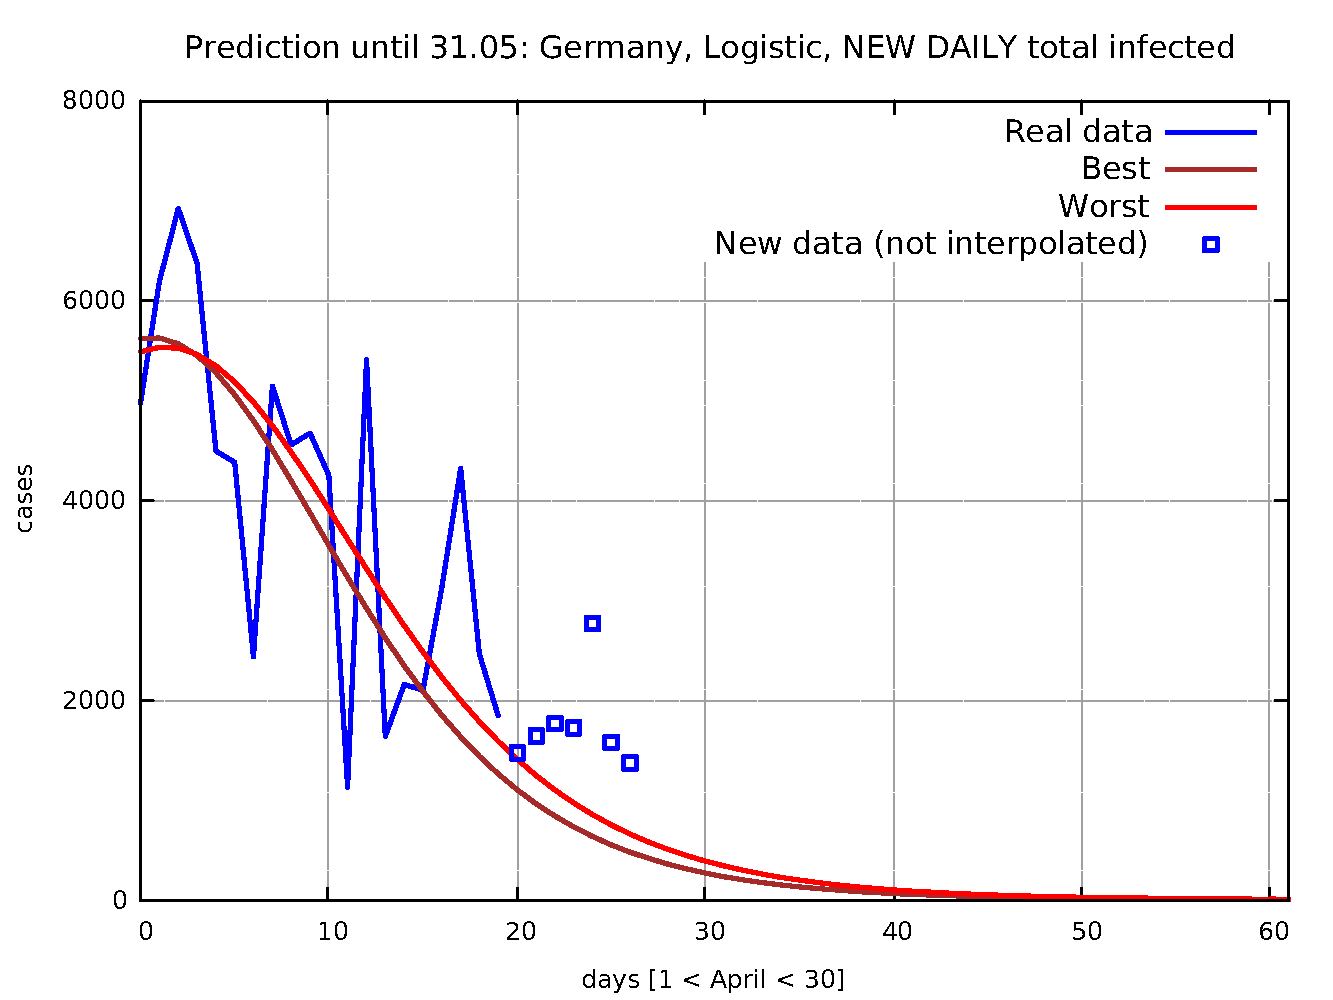
\includegraphics[width=\linewidth]{../de_l_t/peak/peak_prediction.pdf}
  \end{subfigure}
  \caption{Predicting the number of the total \textbf{infected}
	people in \textbf{Germany}
	before the end of May. Results according to the 
	\textbf{simple logistic}
	map; interpolation error of $2\%$.}
\end{figure}


\begin{figure}[h!]
  \centering
  \begin{subfigure}[b]{0.5\linewidth}
  \includegraphics[width=\linewidth]{../it_g_d/posterior.pdf}
  \end{subfigure}
  \begin{subfigure}[b]{0.48\linewidth}
    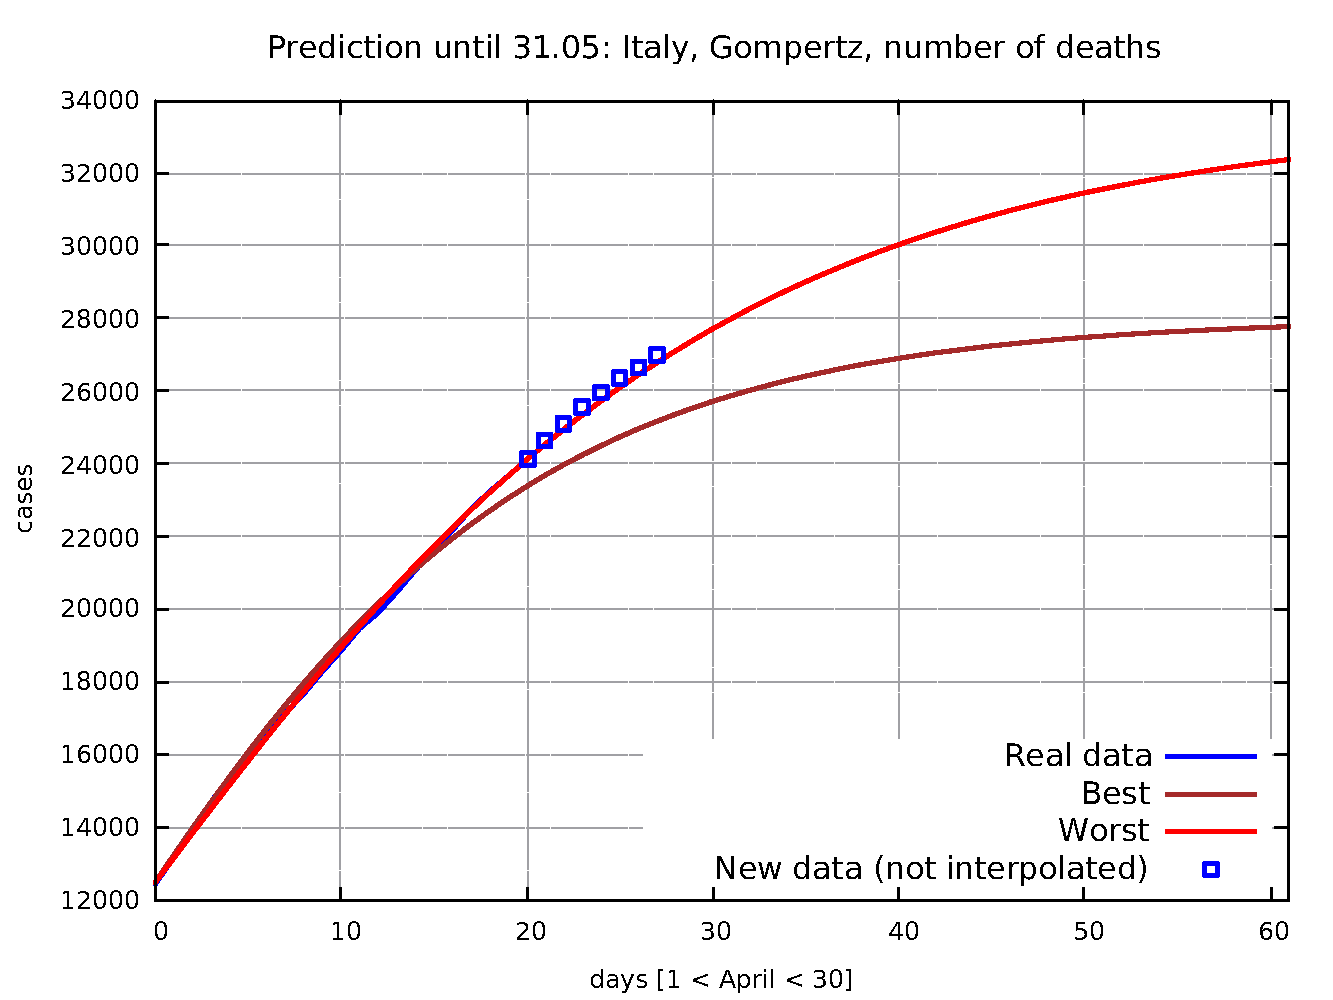
\includegraphics[width=\linewidth]{../it_g_d/prediction.pdf}
  \end{subfigure}
  \begin{subfigure}[b]{0.48\linewidth}
  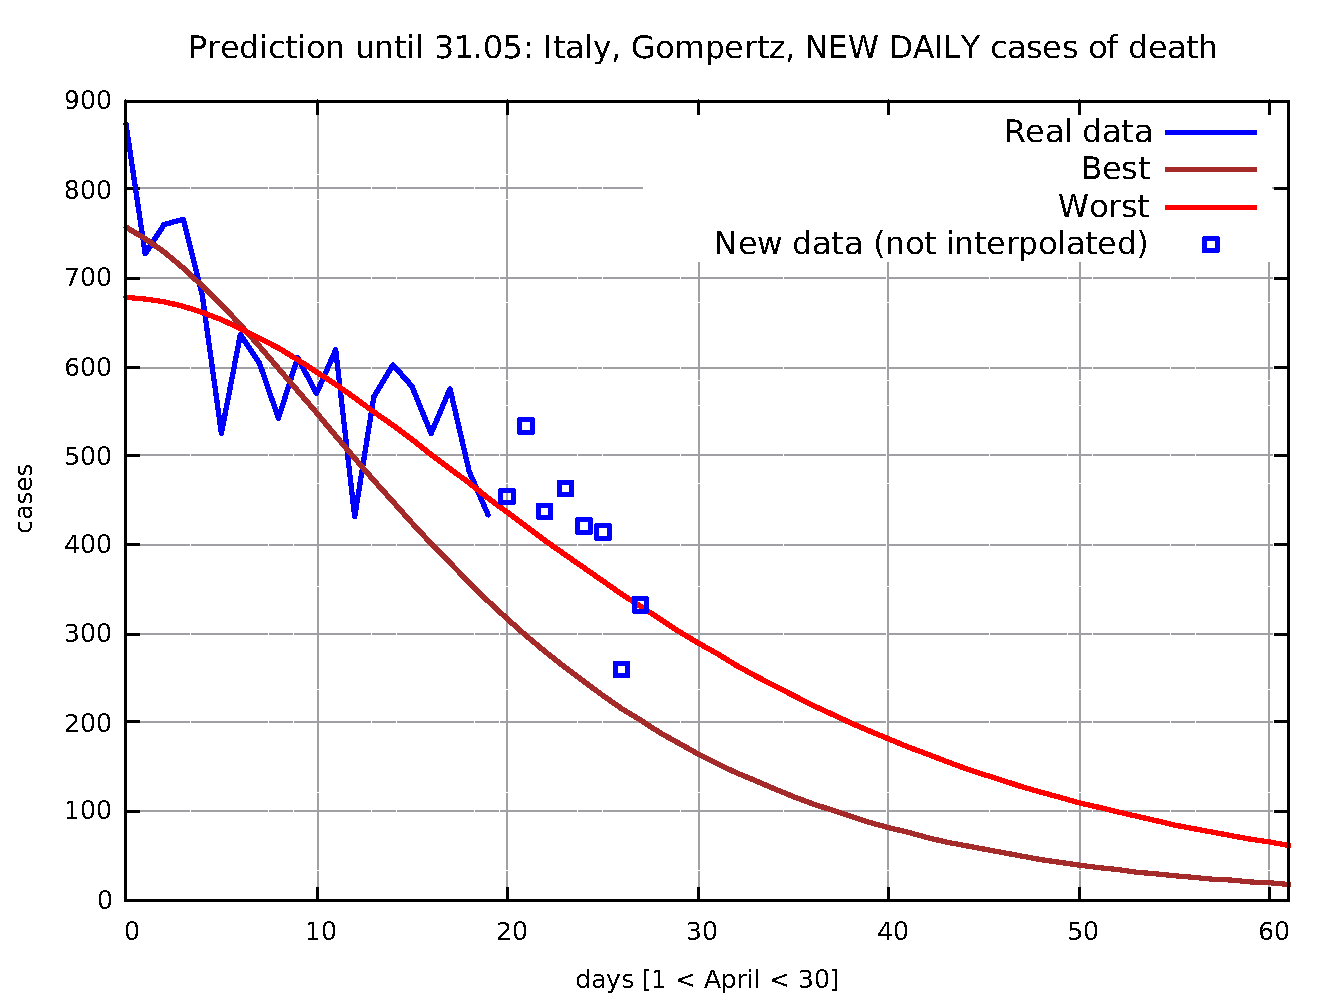
\includegraphics[width=\linewidth]{../it_g_d/peak/peak_prediction.pdf}
  \end{subfigure}
	\caption{Predicting the number of \textbf{deceased}
	people in \textbf{Italy} until the
	end of May. Result according to the \textbf{Gompertz} law, 
	interpolation error around $0.7\%$.}
\end{figure}


\begin{figure}[h!]
  \centering
  \begin{subfigure}[b]{0.5\linewidth}
  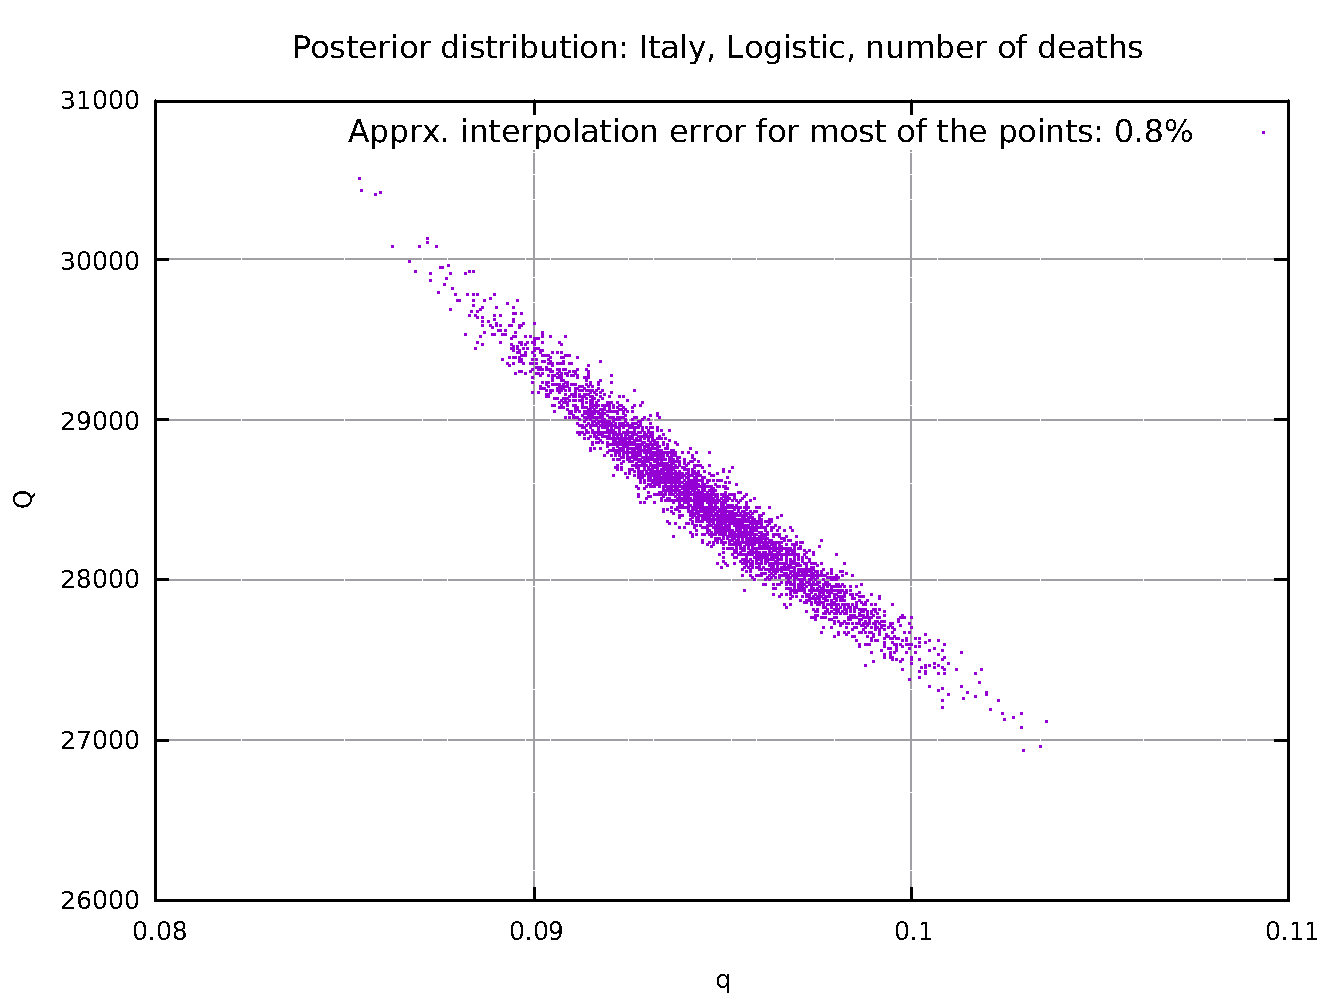
\includegraphics[width=\linewidth]{../it_l_d/posterior.pdf}
  \end{subfigure}  \begin{subfigure}[b]{0.48\linewidth}
    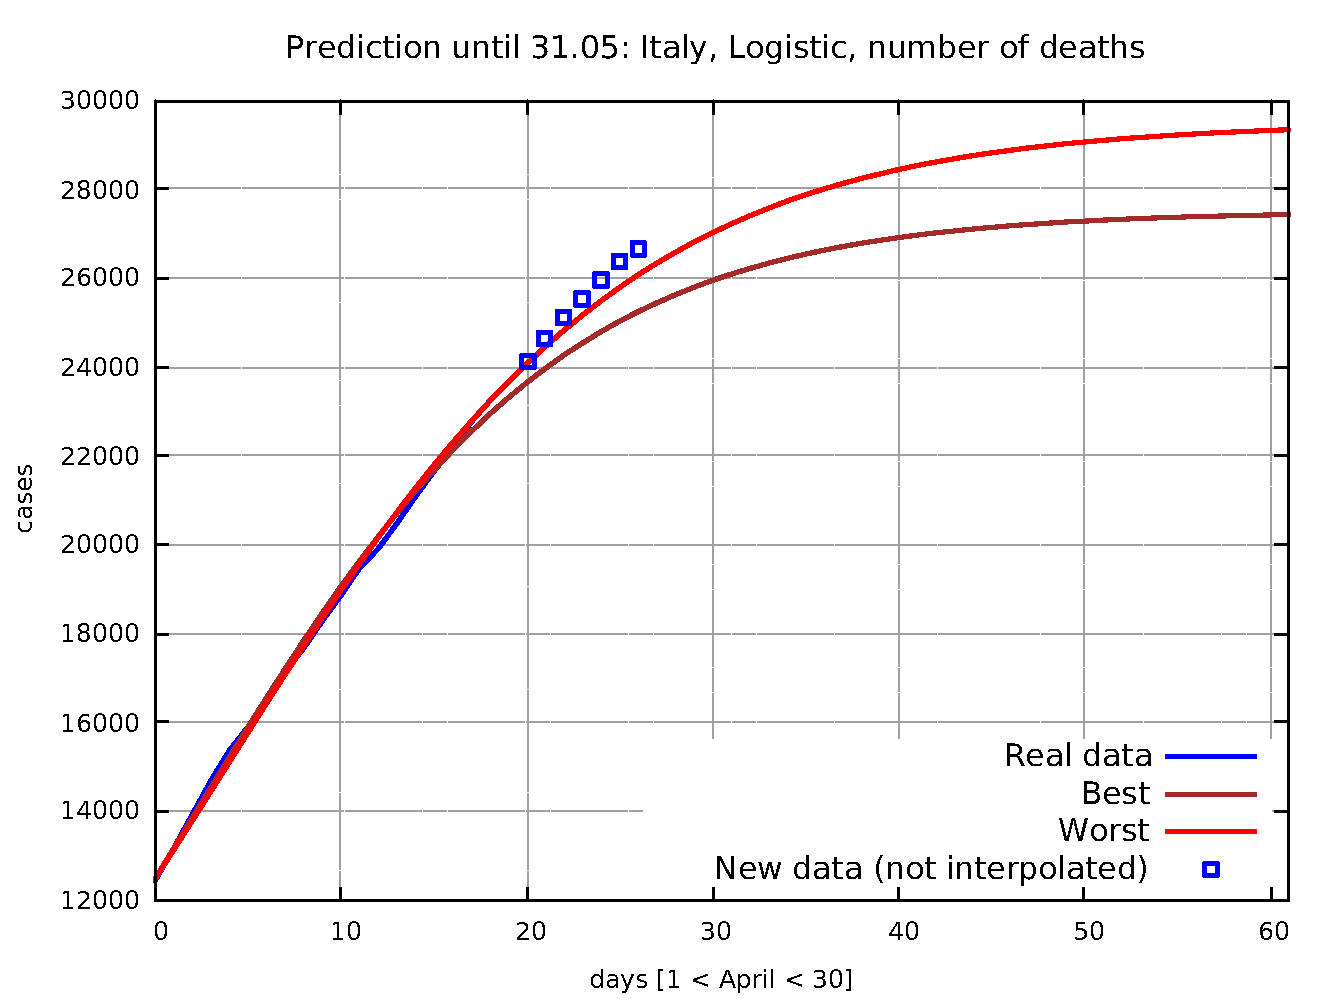
\includegraphics[width=\linewidth]{../it_l_d/prediction.pdf}
  \end{subfigure}
  \begin{subfigure}[b]{0.48\linewidth}
  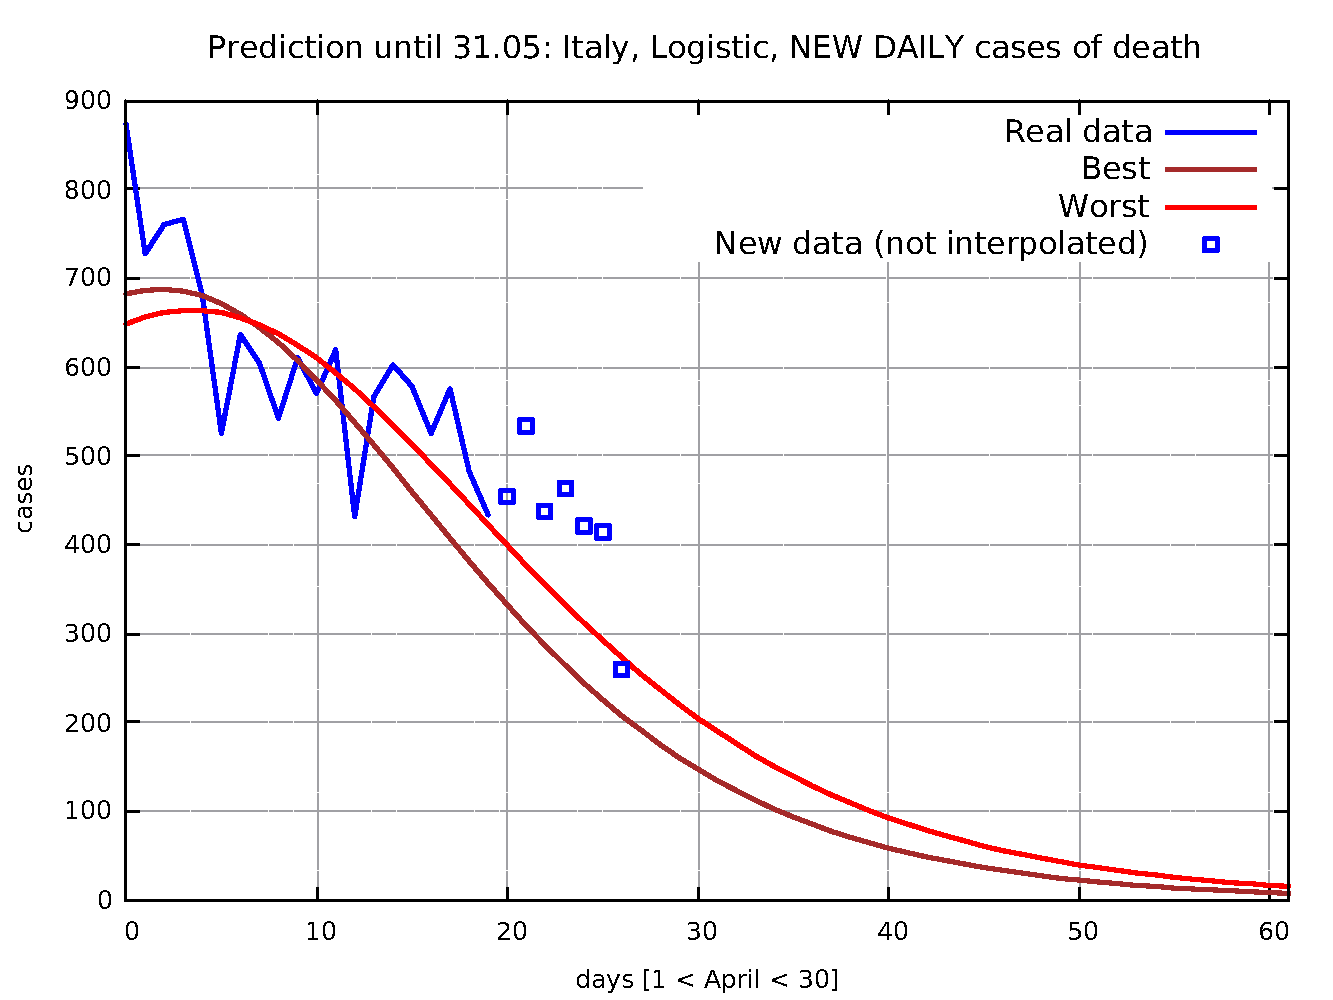
\includegraphics[width=\linewidth]{../it_l_d/peak/peak_prediction.pdf}
  \end{subfigure}
  \caption{Predicting the number of \textbf{deceased}
	people in \textbf{Italy} until the
	end of May. Result according to the \textbf{simple logistic} map
	interpolation error around $0.8\%$.}
\end{figure}

\begin{figure}[h!]
  \centering
  \begin{subfigure}[b]{0.5\linewidth}
  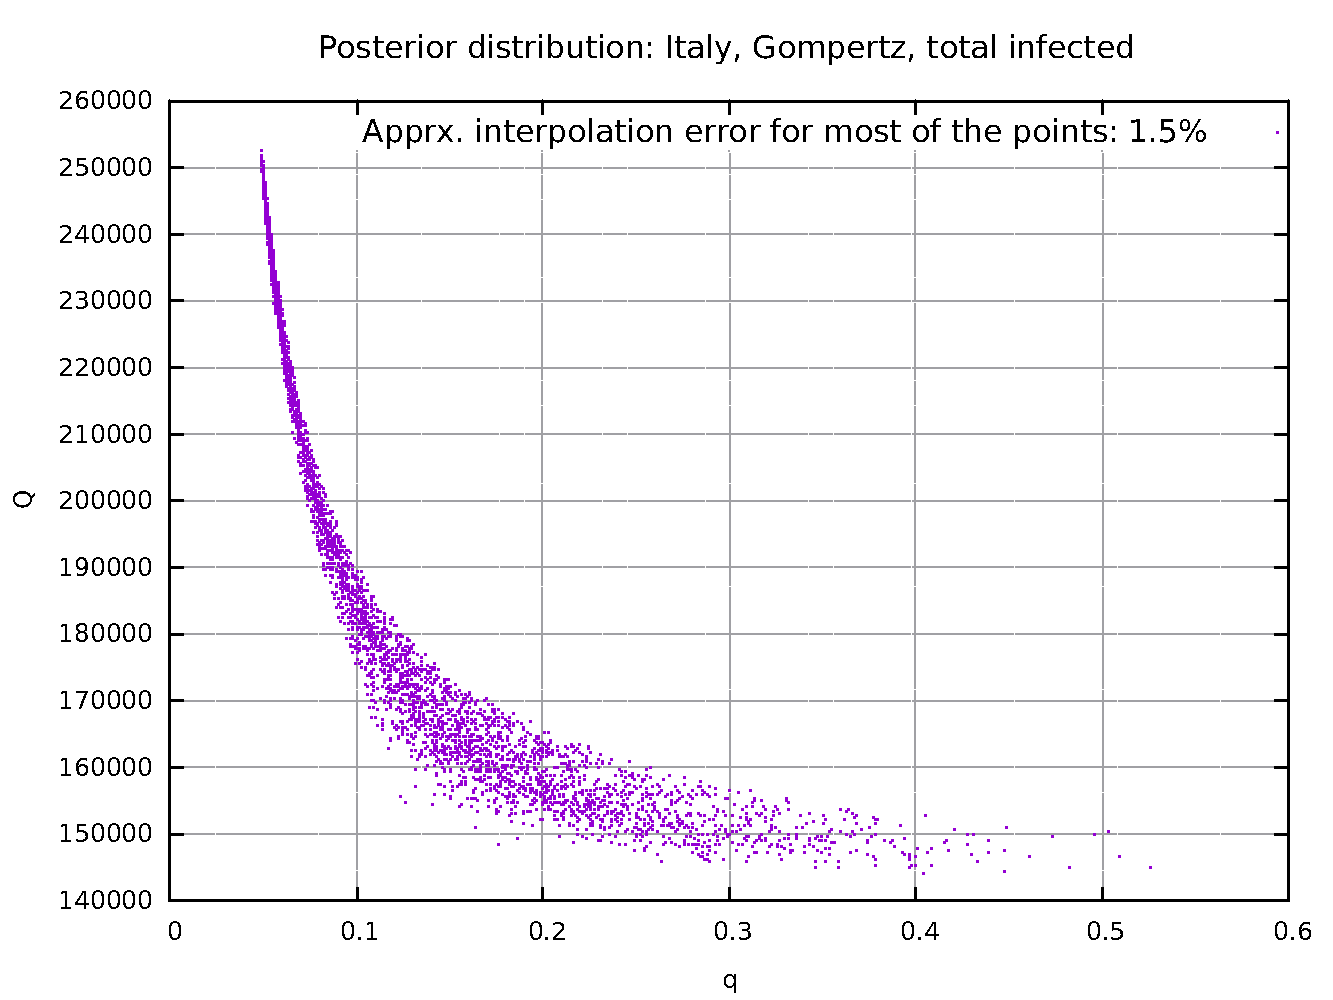
\includegraphics[width=\linewidth]{../it_g_t/posterior.pdf}
  \end{subfigure}
  \begin{subfigure}[b]{0.48\linewidth}
    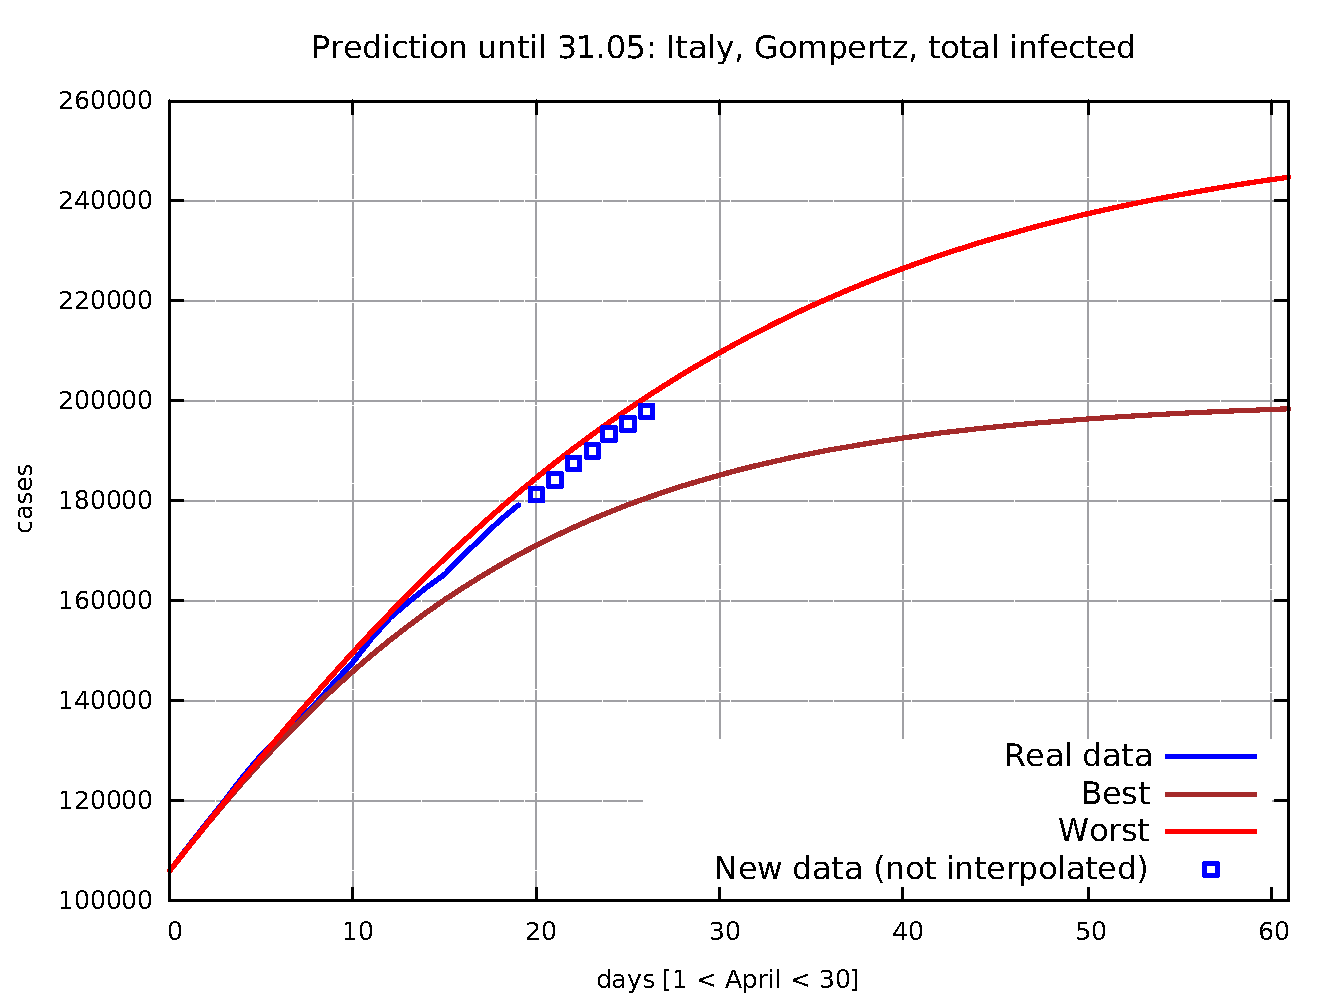
\includegraphics[width=\linewidth]{../it_g_t/prediction.pdf}
  \end{subfigure}
  \begin{subfigure}[b]{0.48\linewidth}
  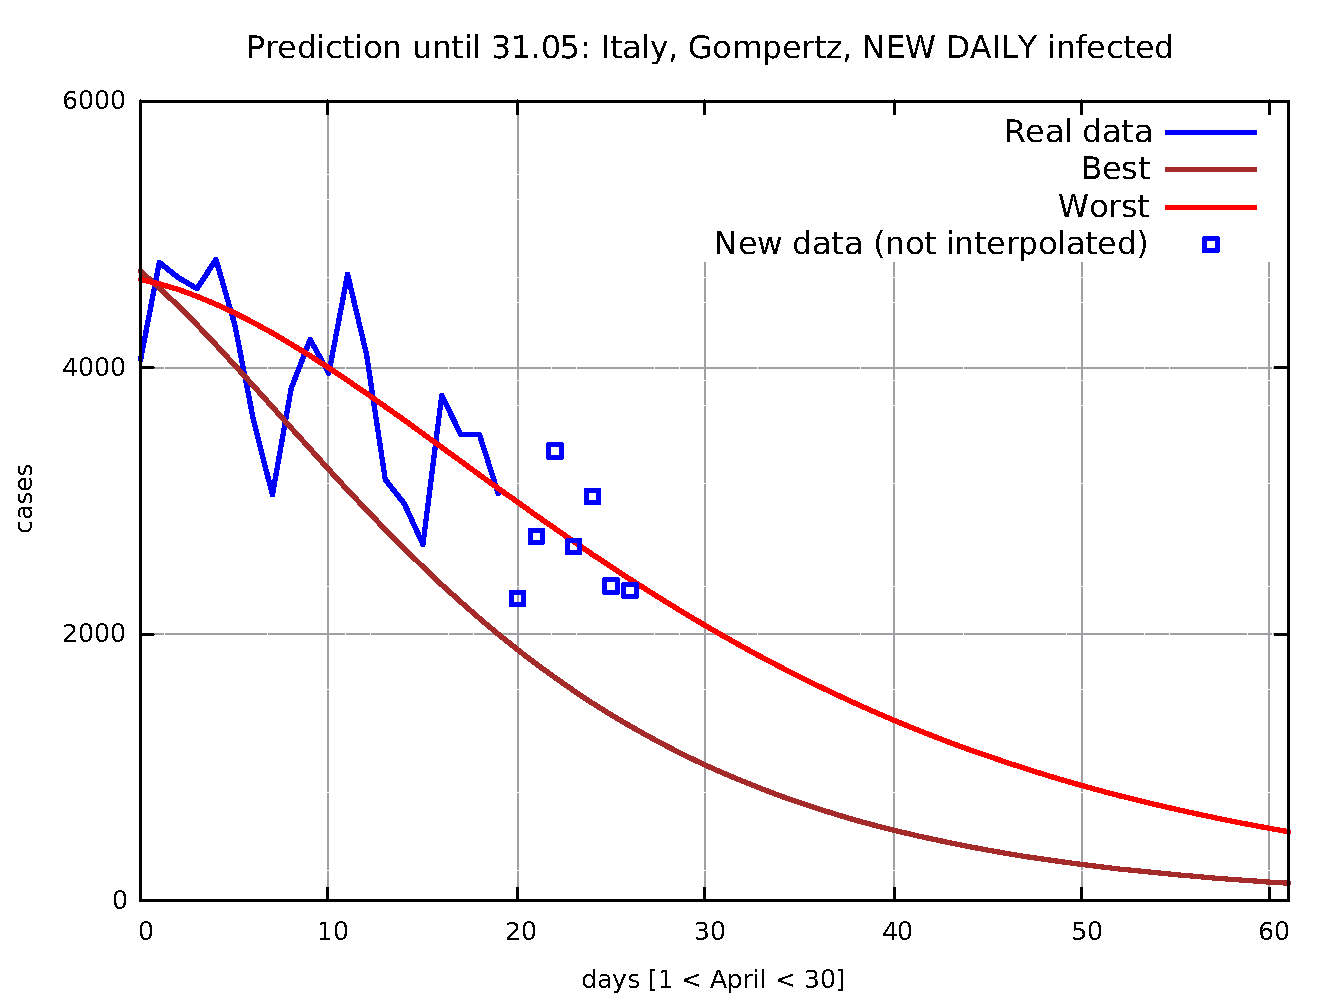
\includegraphics[width=\linewidth]{../it_g_t/peak/peak_prediction.pdf}
  \end{subfigure}
  \caption{Predicting the number of total \textbf{infected}
	people in \textbf{Italy} until the
	end of May. Result according to the \textbf{Gompertz} law,
	interpolation error around $1\%$.}
\end{figure}


\begin{figure}[h!]
  \centering
  \begin{subfigure}[b]{0.5\linewidth}
  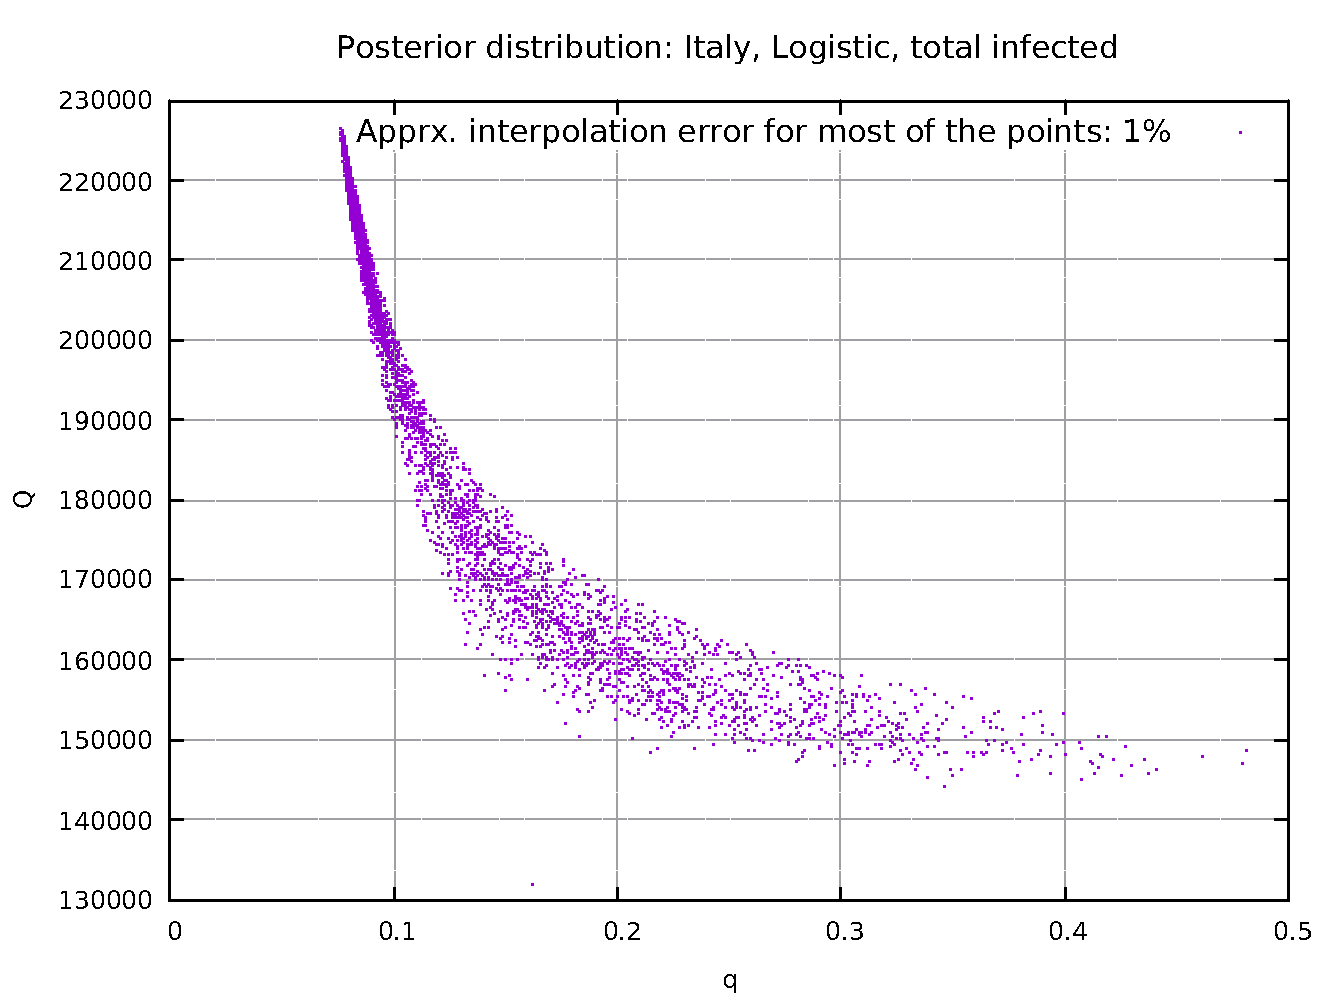
\includegraphics[width=\linewidth]{../it_l_t/posterior.pdf}
  \end{subfigure}  \begin{subfigure}[b]{0.48\linewidth}
    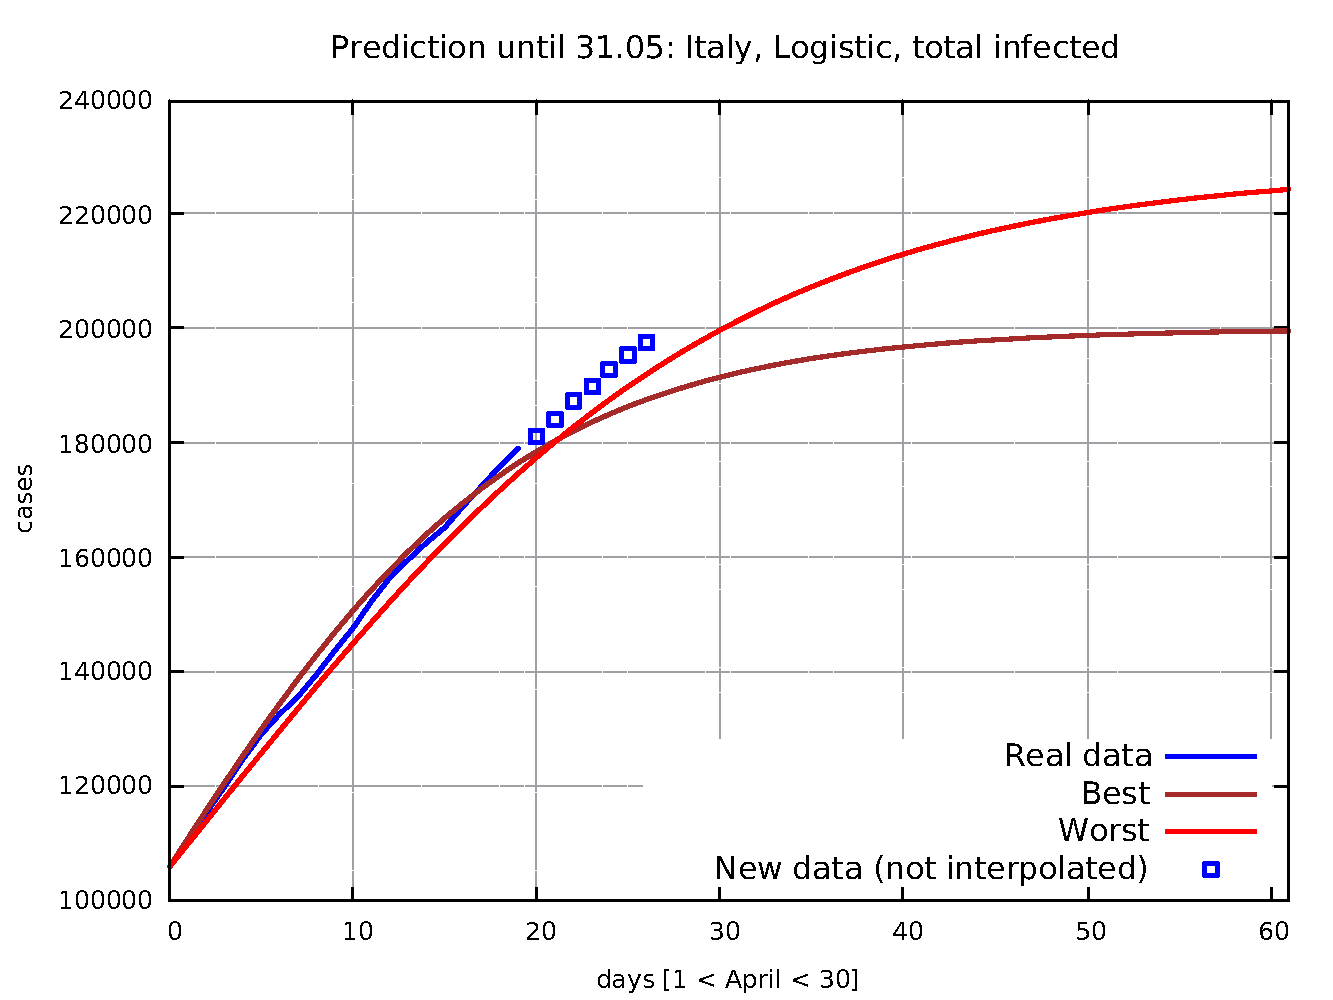
\includegraphics[width=\linewidth]{../it_l_t/prediction.pdf}
  \end{subfigure}
  \begin{subfigure}[b]{0.48\linewidth}
  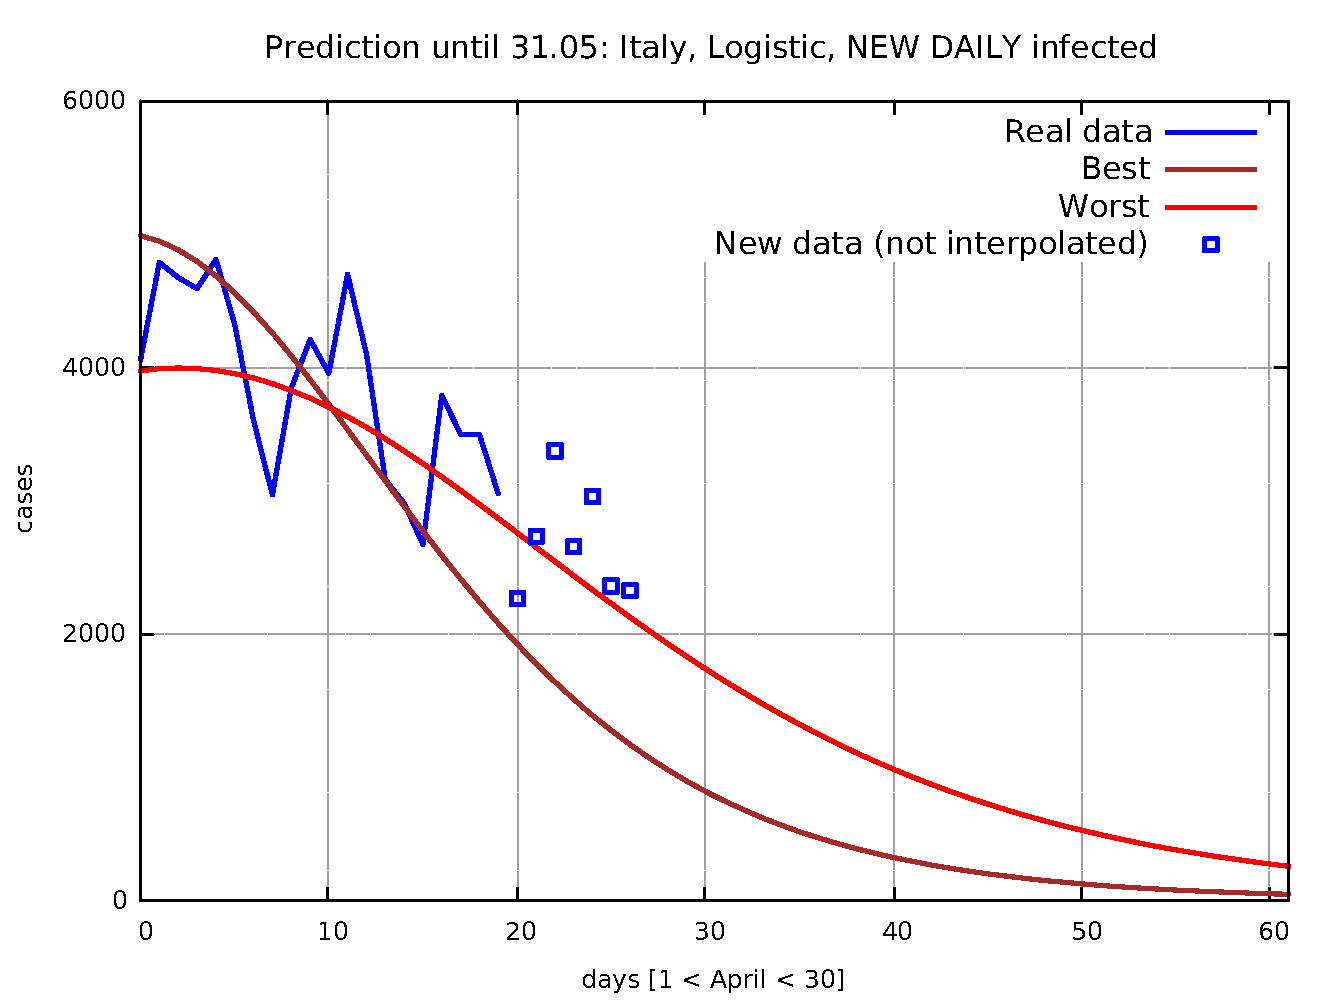
\includegraphics[width=\linewidth]{../it_l_t/peak/peak_prediction.pdf}
  \end{subfigure}
  \caption{Predicting the number of total \textbf{infected}
	people in \textbf{Italy} until the
	end of May. Result according to the \textbf{simple logistic} map,
	interpolation error around $1\%$.}
\end{figure}

\section{Conclusions - TO BE COMPLETELY UPDATED}
Logistic : very bad, as expected...
Generalied Logistic: overfitting? Too many parameters?
Gompertz...promising...

\end{document}
